\chapter{124neV parxkaraNa}

\begin{center}
{\large\rm\bfseries SQUARE AND CUBIC MEASURE}
\vskip .3cm

{\large\bf cadaraLate matutx Gana aLategaLa niNaRya}
\end{center}

\begin{verse}
kaM|| maMdirada goDemaraka | lalxMdadakerekAlepx kUpagAreV kelasa do||LoMdisidaLateya mUlaka| saMdapudeYkUliyava gaLivxvarava peVLevx\char'366||

kaM|| udadxgalaveraDu mAtarxdo| LidadxradaMguNise cadara PalatAnakukxM || udadxgala mALa vadhavA| hodidxda vunanx tavaguNisaladu Gana PalaveY||

vi|| udadxda aLateyanUnx agalada aLateyanUnx guNisidare labadhxvu cadara PalavAgiyU, matutx udadx, agala, ALa, athavA, unanxta ivu mUranunx guNisida labadhx Gana PalavAgiyU iruvadu.
\end{verse}

\begin{center}
{\bf\large hAyxgeMdare.}
\bigskip

\bigskip

\begin{minipage}[t]{6cm}
\renewcommand{\arraystretch}{1.75}
\tabcolsep=.3cm
\begin{tabular}{c|>{\rm}c|>{\rm}c|>{\rm}c|>{\rm}c|c}
\multicolumn{1}{c}{} & \multicolumn{4}{c}{(1neyVdu)} &\\
\multicolumn{1}{c}{} & \multicolumn{5}{l}{$1+1+1+1=4$}\\
\cline{2-5}
\multirow{4}{.3cm}{\rotatebox{270}{udadx aDi}} & 1 & 2 & 3 & 4 & \multirow{4}{.3cm}{\rotatebox{270}{$1+1+1+1=4$}}\\
\cline{2-5}
 & 5 & 6 & 7 & 8\\
\cline{2-5}
 & 9 & 10 & 11 & 12 & \\
\cline{2-5}
 & 13 & 14 & 15 & 16 & \\
\cline{2-5}
\multicolumn{1}{c}{} & \multicolumn{4}{c}{agala aDi} &
\end{tabular}
\end{minipage}
\qquad
\begin{minipage}[t]{6cm}
\renewcommand{\arraystretch}{1.85}
\begin{tabular}{c|>{\rm}c|>{\rm}c|>{\rm}c|>{\rm}c|>{\rm}c|>{\rm}c|c}
\multicolumn{1}{c}{} & \multicolumn{6}{c}{(2neyVdu)} &\\
\multicolumn{1}{c}{} & \multicolumn{6}{l}{$1+1+1+1+1+1=6$}\\
\cline{2-7}
\multirow{3}{.3cm}{\rotatebox{270}{agala aDi 3}} & 1 & 2 & 3 & 4 & 5 & 6 &  \multirow{3}{.3cm}{\rotatebox{270}{$1+1+1=3$}}\\
\cline{2-7}
 & 7 & 8 & 9 & 10 & 11 & 12\\
\cline{2-7}
 & 13 & 14 & 15 & 16 & 17 & 18\\
\cline{2-7}
\multicolumn{1}{c}{} & \multicolumn{6}{c}{udadx aDi $6$} &
\end{tabular}
\end{minipage}
\end{center}

ililx $1$neV AkaqtiyalilxyU matutx $2$neV AkaqtiyalilxyU ira takakx
oMdoMdu manegaLu udadxdalilx $1$ aDi matutx agaladalilx $1$ aDi
iratakakxvugaLAgiyU matutx oMdoMdu cadaraDi visitxVNaRvuLaLxvugaLAgiyU
irutatxveMdu BAvisisutatxde. AdadxriMda $1$neV Akaqtiyalilx udadxda
aLate $4$ aDi $\times$ agalada aLate $4$ aDi = $16$
cadaraDigaLAdavu. hAgeyeV $2$neV A kaqtiyalilx udadx $6$ aDi $\times$
agala $3$ aDi = $18$ cadaraDigaLAdavu. ivugaLa tALeyanunx A
manegaLalilxruva aMkegaLiMda ariya bahudu. 

Gana parimANakAkxdare, meVlina AkaqtigaLanenxV kalulxgaLeMdu BAvisi
varaseyAgi oMdoMdaDi etharxvAdaMthA kalulxgaLanenxV peVrisutAtx
hoVdare, eSaTx, varaseyAguvadoV aSuTx aDi unanxtaveMdu tiLiya beVku.

hAgAdare, meVlina AkaqtigaLa unanxtavu $5$ aDi yeMdeNisikoMDare.
\begin{itemize}
\item[\rm(1)] $4$ aDi udAdx $\times$ $4$ aDi agala $\times$ $5$ aDi
  unanxta $=80$ Gana aDigaLAdavu.

\item[\rm(2)] $6$ aDi udAdx $\times$ $3$ aDi agala $\times$ $5$ aDi
  unanxta $=90$ Gana aDigaLAdavu.
\end{itemize}

hiVgeyeV A AkaqtigaLu $5$ aDi ALavAgi toVDidaMthA tagugxgaLAda
pakaSxdalilx avugaLa Gana parimANavU meVlinaSeTx Agiruvavu.

oMdu veVLe, udadx agala modalAdavugaLalilx aMgulagaLidadxre,
avugaLigelAlx oTiTxge aMgulagaLanenx mADikoMDu guNisabeVku. athavA
BinanxrAshiya meVrige samarAshige taMdukoMDu guNisa bahudu. hAge
baMdaMthA labadhxgaLu cadara aMgulagaLAgidadxre, adanunx hiMdina
koVSaTxkadalilx heVLiruva parxkArakekx $144$riMda BAgisidare,
labadhxvu cadaraDigaLAgiyU sheVSavu cadaraMgulagaLAgiyU
iruvavu. hAyxgeMdare, $25$ aMgula udadx, $8$ aMgula agala idadxre,
$25\times 8=200$ cadaraMgula $\div 144=1$ cadaraDi sheVSa $56$ cadara
aMgulavAyitu. matutx guNisidaMthA \hbox{labadhxvu} Gana aMgulavAgidadxre,
adanunx $1728$riMda BAgisidare labadhxvu GanaDigaLAgiyU sheVSavu
GanaMgulagaLAgiyU iruvavu. hAyxgeMdare, $150$ aMgula udadx $\times 75$
aMgula agala $\times 27$ aMgula ALa $=11250$ Gana aMgulagaLu $\div
1728=6$ Gana aDi, sheVSa $882$ Gana aMgulagaLu Adavu.

inUnx idara tiLavaLike canAnxgi Aga takakx bagUyx samarAshigaLanunx
mADikoLaLxdeV, hAgeV sulaBavAgi guNisuva jAcnxnavuMTATxguvadakUkx
muMde kelavu koVSaTxkagaLu bariyalapxDuvadu. hAyxgeMdare.
\begin{itemize}
\item[\rm(1)] sAdA aMgula $\times$ sAdA aMgula = cadaraMgula

\item[\rm(2)] cadaraMgula $\times$ sAdA aMgula = Gana aMgula

\item[\rm(3)] sAdA aDi $\times$ sAdA aDi = cadaraDi

\item[\rm(4)] cadaraDi $\times$ sAdA aDi = Gana aDi

\item[\rm(5)] $\dfrac{\text{sAdA aDi $\times$ cadaraMgula}}{12}=$ Gana
  aDi sheVSa $\times 144 =$ Gana aMgula 

\item[\rm(6)] $\dfrac{\text{sAdA aMgula $\times$ sAdA aDi}}{12}=$
  cadaraDi sheVSa $\times 12=$ cadaraMgula

\item[\rm(7)] cadaraMgula $\div 144=$ cadaraDi sheVSa cadaraMgula

\item[\rm(8)] cadaraDi $\div 9=$ cadara gaja sheVSa cadaraDi

\item[\rm(9)] Gana aMgula $\div 1728=$ Gana aDi sheVSa Gana aMgula

\item[\rm(10)] Gana aDi $\div 27=$ Gana gaja sheVSa Gana aDi

\item[\rm(11)] sAdA aDi $\times$ cadaraMgula $\times 12=$ Gana aDigaLU
  athavA $\dfrac{\text{sAdA aDi $\times$ cadaraMgula}}{144}=$ Gana aDi
  sheVSa $\times 12$ Gana aMgula

\item[\rm(12)] sAdA aMgula $\times$ cadara aDi =  cadara aDi sheVSa
  $\times 144=$ Gana aMgula

\item[\rm(13)] sAdA gaja $\times$ aDi $\times 3=$ cadaraDi

\item[\rm(14)] sAdA aDi $\times$ sAdA aMgula = labadhx $\div 12=$
  aDigaLu sheVSa $\times 12$ cadaraMgula

\item[\rm(15)] $\dfrac{\text{sAdA gaja $\times$ sAdA aDi $\times$ sAdA
    aMgula}}{4}=$ Gana aDigaLu.
\end{itemize}

ivugaLananunx aritu guNisa bahudu. hAyxgeMdare,

udAharaNe, $1$ gaja $1$ aDi $6$ aMgula udadx, $1$ gaja $2$ aDi $9$
aMgula agala, $3$ gaja $3$ aMgula etharx Adare, adara Gana
parimANaveSuTx?

($1$neV riVti) elalxkekx aMgulagaLanunx mADikoMDu guNisa bahudu.
\begin{center}
\begin{tabular}{lllcrcl}
$1$ gaja & $1$ aDi & $6$ aMgula & = & $56$ & aMgula & udadx\\
$1$ & $2$ & $9$ & = & $69$ & '' & agala\\
$3$ & $0$ & $3$ & = & $111$ & '' & etharx\\[5pt]
\multicolumn{7}{l}{agalu~~\,$56\,\times\, 69\,\times\, 1111=413586\div
  1728=239$ Gana}\\
\multicolumn{7}{l}{\quad aDi, sheVSa $594$ Gana aMgula.}
\end{tabular}
\end{center}

\medskip

($2$neV riVti)
\begin{center}
\begin{tabular}{lllccc}
$1$ gaja & $1$ aDi, & $6$ aM & = & $4\dfrac{1}{2}$ & aDi\\[10pt]
$1$ & $2$ & $9$ & = & $5\dfrac{3}{4}$ & ''\\[10pt]
$3$ & $0$ & $3$ & = & $9\dfrac{1}{4}$ & ''
\end{tabular}
\end{center}
$\dfrac{9}{2}\times\dfrac{23}{4}\times
\dfrac{37}{4}=\dfrac{7659}{32}=239$ Gana aDi sheVSa $\dfrac{11\times
  1728}{32}=594$ Gana aMgula utatxravu. 

\medskip

($3$neV riVti)
\begin{center}
\begin{tabular}{llrccccl}
$1$ gaja & $1$ aDi & $6$ & aM & = & $4$ & aDi & $6$ aMgula\\
$1$ & $2$ & $9$ & '' & = & $5$ & '' & $9$\\
\cline{4-7}
 & & & \multicolumn{4}{c}{$36$} & $54$\\
 & & $20$ & \multicolumn{4}{c}{$30$} & $54$\\
\cline{4-7}
 & & $25$ & \multicolumn{4}{c}{~$6$} & $54$
\end{tabular}
\end{center}

agalu $6$neV koVSaTxka parxkArakekx madhayxda sheVSa $6\times 12=72$
cadaraMgula $+14$ AdadxriMda
\begin{center}
\begin{tabular}{ll@{\qquad}l}
 & $25$ cadara & $126$ cadaraMgula\\[2pt]
etharx $3$ gaja $3$ aMgula = & ~\,$9$ sAdA & ~~~\,$3$ sAdA aM.\\
\cline{2-3}
 & & \\[-7pt]
\multicolumn{2}{r}{
$\left.
\begin{array}{rr}
& 75\\
225 & 1134
\end{array}
\right\}
$}\qquad\, & \raisebox{.4cm}{$378$}
\end{tabular}
\end{center}

\begin{tabular}{rcl}
Iga $12$neV koVSaTxka parxkArakekx $75\div 12$ & = & $6$ Gana aDi
sheVSa $3\times 144$\\
 & = & $432$ Gana aMgulavAyitu,\\
Agalu\hspace{1cm} $6$\hspace{1cm} ''\hspace{1cm} & = & $432$ Gana aMgula
\end{tabular}

\begin{tabular}{rcl}
Iga $11$neV koVSaTxka parxkArakekx $1134\div 144$ &= & $7$ Gana aDi
sheVSa $126$\\[2pt]
$\times 12$ & = & $1512$ Gana aMgula\\
\underline{agalu \hspace{1cm} $7$\hspace{1cm} ''\hspace{1cm}
  $1512$}\\[4pt]
oTuTx \hspace{4.2cm} & \\
\multicolumn{3}{c}{
\begin{tabular}{crl}
$238$ Gana aDi. & $2322$ & Gana aMgula $\div 1728$\\
 $1$~~~~~~~~ & $594$ & Gana aMgula\\
\cline{1-2}
$239$ Gana aDi & $594$ & Gana aMgula utatxravu.
\end{tabular}
}
\end{tabular}


Iga oMdu jagaliyu $8$ gaja udAdx, $6$ aDi agala, $9$ aMgula
etharxvAgidadxre, adara sale eSuTx?

$15$neV koVSaTxkada meVrige $\dfrac{8\times 6\times 9}{4}=108$ Gana
aDigaLu athavA $\div 27=4$ Gana gaja utatxravu.

inUnx koThaDi modalAdavugaLa aLatege.

udAharaNe, $15$ aDi udadx, $12$ aDi $6$ aMgula agala, $8$ aDi etharx
iMthA oMdu koThaDiya goVDegaLige cadara gaja $1$ kekx $4$ ANeV meVrige
baMNA hAkisidare, eSuTx muTuTxvadu?

ililx udadxvanunx etharxdimda guNisidare, oMdu udadx goVDeyasaleyU,
matutx agalavanunx etharxdiMda guNisidare oMdaMgula goVDeya saleyU
Agutatxve. Adare oMdu koThaDige udadxdalilxyU matutx agaladalilxyU
eraDeraDu goVDegaLirutatxve kAraNa udadx goVDegaLa sale
$=2\times\text{udadx}\times \text{etharx}$. matutx agala goDesale $=2\times
\text{agala}\times \text{etharx}$.

Agalu nAlukx goVDegaLa sale $=(2\times\text{udadx}\times
\text{etharx})+(2\times \text{agala}\times \text{etharx})$ Agiruvadu.

AdakAraNa, meVlina leKaKxdalilx $2\times 15$ udadx $\times 8$ aDi
etharx $=240$ udadxda $2$ goVDegaLa sale.
\begin{center}
\begin{tabular}{rcll}
matutx agalada $2$ goVDe $=2\times 12\frac{1}{2}$ aDi agala $\times 8$
aDi & = & $200$\\
\cline{3-3}
nAlukx goVDegaLa sale & & $400$\\
\cline{3-3}
Agalu, dara $4$ ANe meVrige lAgavaDu && $110$ & rU. u. 
\end{tabular}
\end{center}

sUcane|| $\dfrac{\text{Gana aDi}}{\text{udadx $\times$ agala}}=$
etharx, matutx $\dfrac{\text{Gana aDi}}{\text{udadx $\times$
    etharx}}=$ agala, matutx $\dfrac{\text{Gana aDi}}{\text{agala
    $\times$ etharx}}=$ udadx, matutx
$\dfrac{\text{cadaraDi}}{\text{udadx}}=\text{agala}$, matutx
$\dfrac{\text{cadaraDi}}{\text{agala}}=\text{udadx}$. 

I parxkArakekx kaMDu hiDiya bahudu.

udAharaNe, $288$ Gana aDigaLuLaLx oMdu vasutxvina udadxvu $12$ aDi
agalavu $8$ aDi Adare, etharx veSuTx?
\begin{align*}
\text{etharx} &= \frac{288}{28\times 8}=3\text{~ aDi etharx.}\\[5pt]
\text{agala} &= \frac{288}{12\times 3}=8\text{~ agala}.\\[5pt]
\text{udadx} &= \frac{288}{8\times 3}=12\text{~ aDi udAdx.}
\end{align*}
I parxkArakekx tiLadu guNisa beVku.

\bigskip
\begin{center}
{\large\bf dUlada Gana parimANakekx.}
\end{center}
\begin{verse}
kaM|| dUlada sutatxLateyanaM | nAlaroLahxrisutatxlabadx vagiRsutadanaM
|| dUladaniVLadi guNisalf | dUlada Ganamitiyubakukx gaNakaramatadiM||

vi|| dUlada madhayx parxdeVshada sutatxLateyanunx $4$riMda BAgisi BAga
labadxda vagaRvanunx mADi adanunx udadxdiMda guNisa beVku. dUlada
maMda oMdeV samanAgilalxdidadxre, hecucx kaDameyAgiruva
sathxLagaLalilx aLadu A oTaTxnunx sarAsari mADikoMDu leKaKxvanunx mADabeVku.
\end{verse}

udAharaNe, oMdu dUlavu $24$ aDi udadxvAgide. adara sutatxLate
$3\frac{1}{2}$ aDiyAgidadxre, dUlada Gana parimANaveSuTx?

riVti, $\frac{3\frac{1}{2}}{4}=\frac{7}{8}$ vagiRsalu
$\frac{49}{8}\times 3=\frac{147}{8}=18\frac{3}{7}$ Gana aDi utatxra.

idaraMte vanike, rUlf, doMNe, modalAdavugaLa aLateyanunx kaMDu hiDaya
bahudu.

\bigskip
\begin{center}
{\Large\bf 148neV aBayx udAharaNe.}
\end{center}

\begin{itemize}
\item[\rm(1)] $150$ gaja udAdx, $6$ gaja agala, $1\frac{1}{4}$ gaja
  maTaTxvAda hULu maTiTxyanunx tegiyuvadakekx dara Gana gaja $1$ kekx
  $6$ peY meVrige muTuTxvaLi eSATxguvadu?\hfill $35$-$2$-$6$

\item[\rm(2)] $10$ aDi $6$ aMgula udadx, $1$ aDi $3$ aMgula agala, $5$
  aDi $9$ aMgula etatxravAda gAreV goVDege dara Gana aDi $1$kekx $1$
  rUpAyi $8$ ANe meVrige muTuTxvaLi eSATxguvadu?\hfill $113$-$3$-$2$

\item[\rm(3)] $180$ gaja udadx, $7$ aDi agala, $9$ aMgula etatxravAgi
  jalilxV haraDuvadakekx dara $4$ ANeV meVrige muTuTxvaLi eSuTx?\hfill
  $26\frac{1}{4}$

\item[\rm(4)] $16$ aDi udadx, $8$ aDi agalavAda goVDege suMNa
  hacicxsuvadakekx dara cadaraDi $1$kekx $1$ peY meVrige muTuTxvaLi
  eSuTx?\hfill $1$ ANe $\frac{4}{5}$ peY.

\item[\rm(5)] $14$ aDi udAdx, $1$ aDi $2$ aMgula agalavAda maravanunx
  $7$ BAgavAgi koyuyxvadakekx dara rUpAyi $1$ kekx $20$ cadaraDigaLa
  meVrige kUli eSATxguvadu, heVLu?\hfill $13$ ANe $\frac{4}{5}$ peY.

\item[\rm(6)] $5$ aDi udadx, $4$ aDi agala, $3\frac{1}{2}$ aDi
  etharxvuLaLx oMdu peTiTxgeya hora BAgakekx baMNa hAkisuvadakekx
  cadaraDi $1$ kekx $1$ ANe meVrige muTuTxvaLi eSuTx?\hfill utatxra
  $3$ rUpAyi $1$ ANe.

\item[\rm(7)] $60$ cadara gaja $8$ cadaraDi, $18$ cadaraMgulagaLa
  saleyuLaLx oMdu hajArada udadxvu $2$ aDi $6$ aMgulagaLAdare, adara
  agalaveSuTx?\hfill $73$ gaja $2$ aMgula utatxra.

\item[\rm(8)] $2$ gaja pananx vuLaLx oMdu sakalAtige goVTu
  kaTiTxsudadakekx $15$ gaja rubi\char'366\ beVkAgutatxde, Adare A
  sakalAtiya visitxVNaR veSuTx?\hfill $11$ gaja visitxVNaRvu.

\item[\rm(9)] $30$ aDi udAdx, $27$ aDi agalavuLaLx oMdu cikakx maneya
  goVDegaLige kadA hacicxsuvadakekx cadara gaja $1$ kekx $6$ ANeV
  meVrige $57$ rUpAyi muTiTxdare, A maneya etatxra veSuTx?\hfill $12$
  aDi utatxra.

\item[\rm(10)] $20$ gajagaLa udadxvuLaLx oMdu koThaDige hAsuvadakekx
  jaMKAnada beleyu dara cadara gaja $1$kekx $15$ ANe meVrige $28$
  rUpAyi $2$ ANe KacARgutatxde. matutx goVDegaLige kAgada
  hacicxsuvadakekx cadara gaja $1$kekx $9$ ANe meVrige $48\frac{3}{8}$
  rUpAyi KacARgutatxde. Adare A koThaDiya agalaveSuTx?
  udadxveSuTx?\hfill u. agala $1\frac{1}{2}$ gaja. etharx $2$ gaja.

\item[\rm(11)] oMdu keSxVtarxvanunx oMdu koVTiniMdA aLadaMthA
  keSxVtarx Palavu $500$ gajagaLAgiruvadu. adanunx matotxMdu
  koVTiniMda aLadAgeyx $1125$ sale gajagaLAdavu. Adare A eraDu
  koVTugaLa parxmANaveSuTx?

\hfill $1$ gajadudx oMdu. $1\frac{1}{2}$ gajadudx matotxMdu.
\end{itemize}


\chapter{125neV parxkaraNa}

\begin{center}
{\large\rm\bfseries CUBIC MEASURES}
\vskip .3cm

{\large\bf keSxVtarx gaNitagaLanunx kuritadudx.}\\
\vskip .3cm
{\large\bf keSxVtarx BAvagaLa vivaravu.}
\end{center}

\begin{verse}
kaM|| keSxVtarxvu bahuvidhamakukxM| keSxVtarxda BAvaMgaLfLeva tiLivaDasAdhayxM|| keSxVtarxMgaLa KaMDirxsayxdariM| keSxVtarxgaLelalxvanu aLeva mAgaRvapeVLe\char'366
\end{verse}

\begin{center}
keSxVtarxgaLanunx KaMDirxsuva vidhiyu.
\end{center}

\begin{verse}
kaM|| samanAdaMkara Bujega| LakxrXmavAgirutipaR viSama catura
sarxMga|| Lasxma viSamAdi tirxBujega| Lamaruva vatuRLagaLAgi
KaMDirxsukeSxVtarxM|| 
\end{verse}

\newpage

{\bf keSxVtarx BAvagaLu matutx avugaLa hesarugaLanunx kuritadudx.}
\begin{figure}[H]
\centering
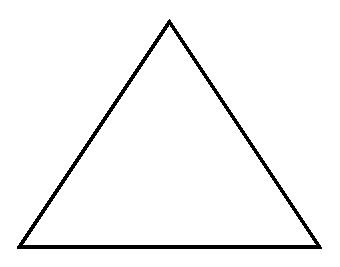
\includegraphics[scale=.75]{figure/fig1.eps}
\end{figure}
idu samatirxBujeyu. aMdare, adara mUru BAvagaLu samagaLAgi uLaLxdudx.
\begin{figure}[H]
\centering
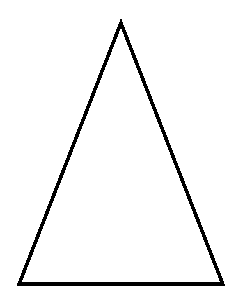
\includegraphics[scale=.75]{figure/fig2.eps}
\end{figure}
idu samadivxbAhu tirxBujeyu. aMdare, adara eraDu bAvugaLu samagaLAgi
uLaLxdudx. 
\begin{figure}[H]
\centering
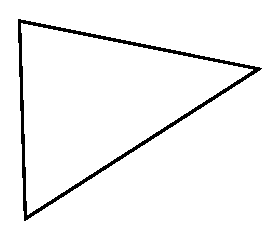
\includegraphics[scale=.75]{figure/fig3.eps}
\end{figure}
idu viSamatirxBujeyu. aMdare, samavalalxda mUru bAhugaLuLaLxdudx.
\begin{figure}[H]
\centering
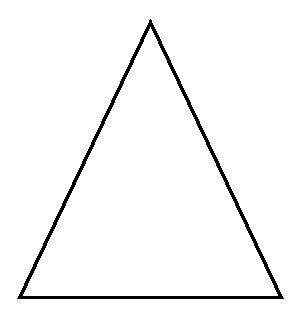
\includegraphics[scale=.65]{figure/fig4.eps}
\end{figure}
idu laGu koVNa tirxBujeyU. aMdare, mUru koVNagaLU laGutaravAgiruvavu.
\begin{figure}[H]
\centering
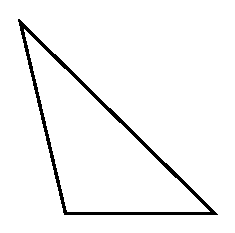
\includegraphics[scale=.75]{figure/fig5.eps}
\end{figure}
idu vishAlakoVNa tirxBujeyu. aMdare, adara oMdu koVNavu samakoVNakiMtA
adhikavAgiruvadu.
\begin{figure}[H]
\centering

\includegraphics[scale=.7]{figure/fig6.eps}
\end{figure}
idu samakoVNa tirxBujeyu. aMdare, idara oMdu koVNavu
samakoVNavAgiruvadu.
\begin{figure}[H]
\centering
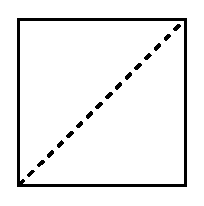
\includegraphics[scale=.7]{figure/fig7.eps}
\end{figure}
idu sama catuBuRjeyu. aMdare, idara bAhugaLelAlx samagaLAgiyU
koVNagaLu sama koVNagaLAgiyU uLaLxdudx, idanunx cacAcxka veMtalU,
vagaR keSxVtarxveMtalU heVLutAtxre.
\begin{figure}[H]
\centering

\includegraphics[scale=.75]{figure/fig8.eps}
\end{figure}
idu Aya keSxVtarxvu. aMdare, koVNagaLelAlx samakoVNagaLAgiyU, aBi
muKavAda bAhugaLu samanAMtara\-vuLaLxvugaLAgiyU irutatxve.

\vfill\eject

\begin{figure}[H]
\centering
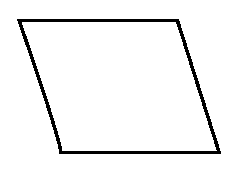
\includegraphics[scale=.8]{figure/fig9.eps}
\end{figure}
idu viSama koVNa, samacatuBuRjeyu. aMdare, adara bAhugeLelAlx
samavAgidudx koVNagaLu sama koVNagaLalalxdeV iruvavU.
\begin{figure}[H]
\centering
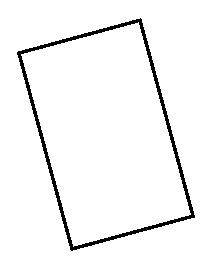
\includegraphics[scale=.8]{figure/fig10.eps}
\end{figure}
idu viSamAyatavu. aMdare, aBimuKa bAhugaLu oMdakokxMdu samavAgiyU
koVNagaLelAlx samavalalxdavugaLAgiyU iruvavU.
\begin{figure}[H]
\centering
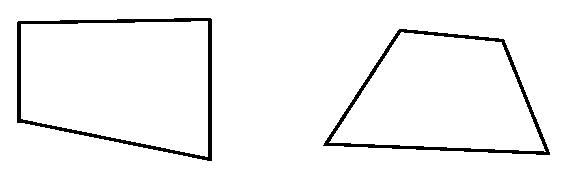
\includegraphics[scale=.8]{figure/fig11.eps}
\end{figure}
itAyxdigaLelAlx viSama catuBuRjegaLeMdu tiLiya takakxdudx.
\begin{figure}[H]
\centering
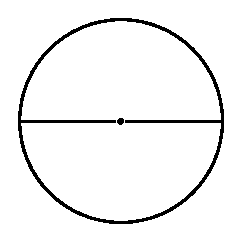
\includegraphics[scale=.8]{figure/fig12.eps}
\end{figure}
idu vatuRLa keSxVtarxvu. aMdare, paridhi yeMba oMdu reVKeyiMda
sutatxlapxTiTxruvadu. I keSxVtarxda sutatxLateyanunx paridhiyeMtalU,
madhayxda biMduvanunx keVMdarxveMtalU, A keVMdarx mAgaRvAgi vAyxpisi
eraDu pAshavxRgaLalilxyU paridhiyanunx muTiTxruva saraLa reVKeyanunx
vAyxsaveMtalU tiLiya beVku.

\eject

\begin{figure}[H]
\centering

\includegraphics[scale=.8]{figure/fig13.eps}
\end{figure}
idaralilx madhayx biMduviniMda paridhi varigU vAyxpisiruva saraLa
reVKeyanunx tirxjAyx eMtalU adhaR vAyxsaveMtalU heVLutAtxre.
\begin{figure}[H]
\centering
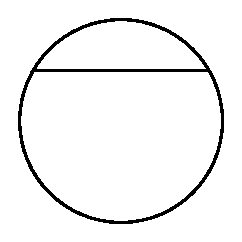
\includegraphics[scale=.8]{figure/fig14.eps}
\end{figure}
idaralilxruva saraLa reVKeyanunx jAyx yeMtalU adara yeraDu koneyanunx
sAdhisira takakx soTaTx reVKeyanunx AvaraNeyeMtalU dhanuveMtalU
heVLutAtxre. matutx A jAyx yeMba saraLa reVKeyiMda CeVdisalapxTaTx
BAgadavxyavanunx vaqtatxda KaMDaveMtalU tiLiya beVku.
\begin{figure}[H]
\centering
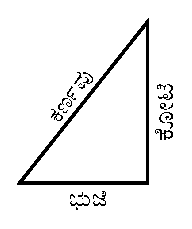
\includegraphics[scale=.9]{figure/fig15.eps}
\end{figure}
idaralilx samakoVNina aBimuKavAgiruva saraLa reVKe athavA bAhuvanunx
kaNaRveMtalU, uLida eraDu bAhugaLige Buje koVTi eMtalU tiLiyabeVku.
\begin{figure}[H]
\centering
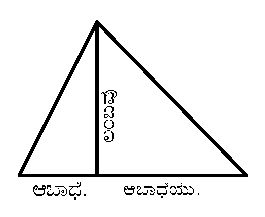
\includegraphics[scale=.9]{figure/fig16.eps}
\end{figure}
idaralilx meVlina koVNadiMda keLagina bAhuvinavarege ira takakx saraLa
reVKeyanunx laMbaveMtalU niVLaveMtalU adu niMtiruva bAhuvige
pAdaveMtalU A laMba reVKeya Ace Ice iratakakx pAdada KaMDagaLanunx
AbAdhe eMtalU tiLiya beVku.

\eject

{\bf eMthA rUpavAda keSxVtarxgaLanAnxdarU KaMDirxsuva mAgaRvu.}

\begin{figure}[H]
\centering
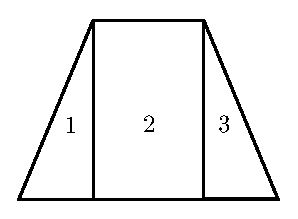
\includegraphics[scale=.75]{figure/fig17.eps}
\end{figure}

idanunx CeVdisalAgi $1$, $3$neV AkaqtigaLuLaLx eraDu tirxBujegaLUnu $2$neV
AkaqtiyAda oMdu catuBuRjeyU uMTAdavu.

\begin{figure}[H]
\centering
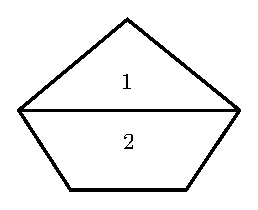
\includegraphics[scale=.75]{figure/fig18.eps}
\end{figure}

idanunx CeVdisalAgi $1$ neVdu tirxkoVNavU $2$ neVdu catuBuRjeyU
uMTAdavu.

\begin{figure}[H]
\centering
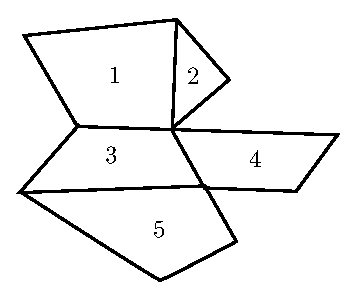
\includegraphics[scale=.75]{figure/fig19.eps}
\end{figure}

idanunx CeVdisalAgi $1$, $3$, $4$, $5$ catuBuRja keSxVtarxgaLU $2$ neV
tirxkoVNa keSxVtarxvU uMTAdavu.

ivugaLa aLategaLiMda keSxVtarx PalagaLanunx muMde heVLuva sUtarxgaLa
parxkArakekx mADa bahudu.

inunx eSuTx vakarxgaLAda BUmigaLidAdxgUyx avugaLanunx ideV upAyavAgi
KaMDirxsab beVku.


\chapter{126neV parxkaraNa}

\begin{center}
{\large\bf keSxVtarx PalagaLanunx kuritadudx.}
\vskip .3cm

{\large\bf tirxBujegaLa keSxVtarx PalagaLanunx kANuva riVtiyu.}
\vskip .3cm

{\large\bf sUtarx.}
\end{center}

\begin{verse}
kaM|| pAdada aLateya mADuta| pAdadedamURleyiMda niVLavanaLeyuta||
lAdara diridava \hbox{nadhiRsa|} lAdude PalakeSxVtarx sakala
tirxBujaMgaLiguM||

vi|| tirxBujegaLa pAdada aLateyanunx mADi adariMda niVLa daLateyanunx
guNisi adhiRsidare, baruva labadhxveV AyAya tirxBuje keSxVtarxgaLa
PalagaLAgiruvavu. 
\end{verse}

\begin{center}
{\bf udAharaNe.}
\end{center}

\begin{figure}[H]
\centering
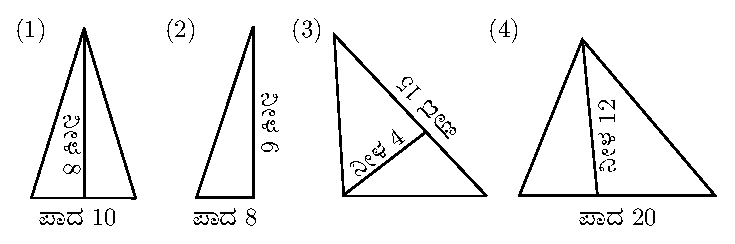
\includegraphics{figure/fig20.eps}
\end{figure}

AgalU
\begin{itemize}
\item[\rm(1)] $\dfrac{10\times 8}{2}=40$ idu $1$neV Akaqtiya keSxVtarx Palavu.

\item[\rm(2)] $\dfrac{8\times 6}{2}=24$ idu $2$neV Akaqtiya keSxVtarx Palavu.

\item[\rm(3)] $\dfrac{15\times 4}{2}=30$ idu $3$neV Akaqtiya keSxVtarx Palavu.

\item[\rm(4)] $\dfrac{20\times 12}{2}=120$ idu $4$neV Akaqtiya
  keSxVtarx Palavu.
\end{itemize}

\newpage

\begin{center}
{\large\bf viSama modalAda catuBuRjegaLa keSxVtarx PalagaLanunx kANuva
  riVti.}
\medskip

{\large\bf sUtarx}
\end{center}

\begin{verse}
kaM|| koVNatarxyadA kaqtiga| LokxVNa catuSaTxyadoLadhaR parimiti
sidadhxM|| koVNa catuSaTxya melalxva| koVNatarxya mADukaLadu
peVLeYsulaBaM||

vi|| nAlukx koVNagaLuLaLx AkaqtigaLelAlx eraDu tirxkoVNa kaqtigaLa
parimANagaLige samAnagaLAgiyU athavA elAlx tirxkoVNagaLU catuBuRja
keSxVtarxgaLalilx adhaR parimANagaLige
samAnagaLAgiratakakxdu. savxtashishxdadhxgaLAdadxriMda eMthA
catuBuRjegaLanAnxdarU eraDu tirxkoVNagaLAgi KaMDirxsi meVle heVLiruva
tirxkoVNa keSxVtarxgaLa aLateyaMteV keSxVtarx PalagaLanunx sulaBavAgi
sAdhisikoLaLx bahudu.\qquad hAyxgeMdare. 
\begin{figure}[H]
\centering
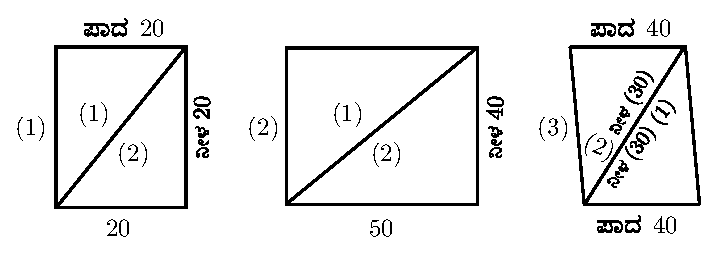
\includegraphics{figure/fig21.eps}
\end{figure}
\begin{figure}[H]
\centering
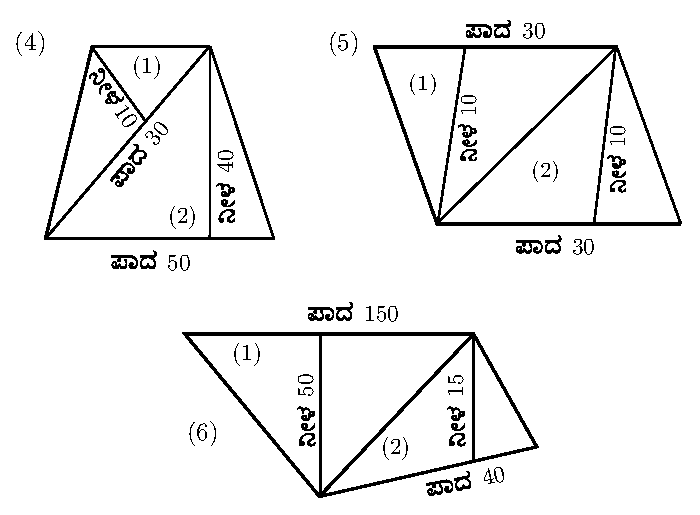
\includegraphics{figure/fig22.eps}
\end{figure}
\end{verse}

\begin{itemize}
\item[\rm(1)] 
\begin{tabular}[t]{rcl}
$\dfrac{20\times 20}{2}=$ & $200$ & idu $1$neV tirxBuja keSxVtarx Palavu.\\[15pt]
$\dfrac{20\times 20}{2}=$ & $200$ & idu $2$neVdara Palavu.\\
\cline{2-2}
oTuTx & $400$ & idu $1$neV Akaqtiya oTuTx keSxVtarx Palavu.
\end{tabular}
\end{itemize}

\begin{verse}
sU|| I cacAcxka keSxVtarxda yAvadAdarU oMdu bAhuvina aLateyanunx
vagiRsidarU athavA yAvadAdarU eraDu bAhugaLanunx guNisidarU keSxVtarx
PalagaLAguvavu. 
\end{verse}

\begin{itemize}
\item[\rm(2)] $50\times 40=2000$ idu $2$neV Akaqtiya Palavu

\item[\rm(3)]
\begin{tabular}[t]{rrl}
$\dfrac{40\times 30}{2}=$ & $600$ & idu $1$neV keSxVtarx tirxkoVNada
Palavu\\[8pt]
$\dfrac{40\times 30}{2}=$ & $600$ & idu $2$neV tirxBuja
keSxVtarxPalavu\\
\cline{2-2}
 & $1200$ & idu $3$neV Akaqtiya oTuTx keSxVtarxPalavu.
\end{tabular}

\item[\rm(4)]
\begin{tabular}[t]{rrl}
$\dfrac{30\times 10}{2}=$ & $150$ & idu $1$neV tirxkoVNada Palavu\\[8pt]
$\dfrac{50\times 40}{2}=$ & $1000$ & idu $2$neV tirxkoVNada Palavu\\
\cline{2-2}
 & $1150$ & idu $4$neV Akaqtiya oTuTx keSxVtarxPalavu.
\end{tabular}

\item[\rm(5)]
\begin{tabular}[t]{rrl}
$\dfrac{30\times 10}{2}=$ & $150$ & idu $1$neV tirxkoVNada
Palavu\\[8pt]
$\dfrac{30\times 10}{2}=$ & $150$ & idu $2$neV tirxkoVNa Palavu\\
\cline{2-2}
 & $300$ & idu $5$neV Akaqtiya oTuTx keSxVtarx Palavu.
\end{tabular}

\item[\rm(6)]
\begin{tabular}[t]{rrl}
$\dfrac{150\times 50}{2}=$ & $27500$ & idu $1$neV tirxkoVNa keSxVtarx
Palavu\\[8pt]
$\dfrac{40\times 15}{2}=$ & $300$ & idu $2$neV tirxkoVNada Palavu\\
\cline{2-2}
 & $27800$ & idu $6$neV Akaqtiya oTuTx keSxVtarx Palavu.
\end{tabular}
\end{itemize}

\newpage

\begin{center}
{\bf\LARGE 126neV parxkaraNa.}\\
\vskip .3cm
{\large\bf vaqtatx keSxVtarx Pala, goVLa kaMtuka jAla Pala, matutx
goVLa gaBaR}\\
\vskip .3cm
{\large\bf Gana Pala paridhi sAdhana modalAdavugaLanunx kuritu.}
\end{center}

\begin{figure}[H]
\centering
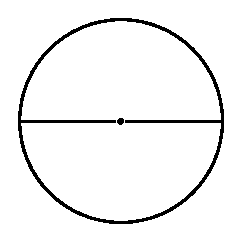
\includegraphics{figure/fig12.eps}
\end{figure}

I paridhiya aLateyanunx pAkadiMdalAgaliV kASaTxdiMdalAgaliV
niNaRyavAgi aLiya takakxdudx asAdhayxvAgiruvadadxriMda adakAkx
vAyxsada parimANadiMdaleV sUkaSxmX, matutx sUthxla paridhigaLa
aLateyanunx sAdhisikoLaLx bahudu. hAyxgeMdare,

\medskip
\begin{center}
{\large\bf sUtarx.}
\end{center}

\begin{verse}
kaM| vaMdu vAyxsakekx mUruM| aMdayutadoLAruvaMdu manuBAgagaLU||
eMdigirutihadu sUkaSxmXdo| LeMdariparidhi parxmANa gaNakaramatadiM||

sUthxla mAgaRkekx. kaM|| ELakikxpapxtetxraDadu| tALiruvadu
sUthxlaparidhi eMdaritadanaM|| meVLisiteYrXrAshiyapari|
yoVLihavAyxsakekxtakakx paridhiyanoVDeY||


vi|| oMdu vAyxsakekx $3.1416$ sUkaSxmX paridhi parxmANavU. $7$
vAyxsakekx $22$ sUthxla paridhi parxmANavu, iruvadadxriMda eSuTx
vAyxsakekx beVkAdarU terxYrAshi gaNitadaMte paridhigaLanunx kaMDu
hiDiya bahudu.
\end{verse}


\medskip

\begin{center}
{\large\bf vaqtatx keSxVtarx Palavanunx kuritadudx.}
\medskip

{\large\bf sUtarxgaLu.}
\end{center}

\begin{description}
\item[\textmd{kaM||} \rm(1)] vaqtatxda paridhiyanadhiRsi matatxda
vAyxsAthaRdiMda guNisalaPxlavuM|| ititxha vAyxsavanogiRsi|
matatxyutadi\-nAlukx yeYdeMTeVLaroLiriyeY||

\item[\rm(2)] paridhiya vAyxsadoLiriyuta| sarigadanAlABxgamADu
sUkaSxmXdaLate gaM|| pariyaritu vAyxsadogaRva| nirikaraNi\-doLahxrisu
manuvinoLagadu sUthxlaM||

\item[\rm(3)] vAyxsAdhaRdavagaRvanaM| leVsenipAmUru rUpaveVLaroMdaM||
vAsara vilalxde guNisalf| leVshavu tapipxlalx sUthxla vaqtatxda
Palavu||
\end{description}

\begin{description}
\item[\textmd{vi||} \rm(1)] 
vaqtatxda paridhiyanunx adhiRsi adanunx vAyxsAdhaRdiMda guNisidare,
vaqtatx keSxVtarx Pala baruvadu.

\item[\rm(2)] vAyxsavanunx vagiRsi adanunx $.7854$ I dashAMshadiMda
guNisidare, keSxVtarxPala baruvadu.

\item[\rm(3)] paridhiyanunx vAyxsadiMda guNisi nAlakxriMda BAgisidare,
vaqtatx keSxVtarx Pala baruvadu.

\item[\rm(4)] vAyxsada vagaRvanunx $11$riMda guNisi $14$ BAgisidare,
savxlapx sUthxlavAgi keSxVtarx Pala baruvadu.

\item[\rm(5)] vAyxsAdhaRda vagaRvanunx $3\frac{1}{7}$riMdA guNisidare,
sUthxlavAgi vaqtatx keSxVtarxPala baruvadu.
\end{description}

hAyxgaMdare. meVlina vaqtatxda vAyxsavu $12$ idadxre, adara
paridhiyanUnx keSxVtarx PalavanUnx kaMDu hiDi?

\medskip

riVtiyu {\rm(1)} vAyxsa $12\times 3.1416=37.6992$ idu paridhi
parxmANavu. matutx {\rm(2)} $7$ vAyxsakekx : $22$ paridhi $::\;12$
vAyxsakekx $=\frac{261}{7}=37\frac{5}{7}$ sUthxla paridhiyu.

\medskip
\begin{center}
{\bf keSxVtarx Palakekx riVti.}
\end{center}

\begin{itemize}
\item[\rm(1)]
\begin{tabular}[t]{cc}
paridhi. & vAyxsa.\\
$37.6992$ & $12$\\
adhiRsalu &
\end{tabular}

$18.8496\times 6=113.0976$ idu sUkaSxmXvAda keSxVtarx Palavu.

\item[\rm(2)] $12$ vAyxsavu, vagiRsalu $144\times .7854=113.0976$ idU
sUkaSxmXvAda keSxVtarx Palavu.

\item[\rm(3)] paridhi $37.6992\times 12$ vAyxsa $=452.3904\div
4=113.0976$ idU sUkaSxmXvAda keSxVtarx Palavu.

\item[\rm(4)] vAyxsa $12$ra vagaRvu $\frac{72\times
11}{7}=\frac{792}{7}=113\frac{1}{7}$ idu sUthxla keSxVtarx PalavU.

\item[\rm(5)] sUthxla paridhi $37\frac{5}{7}=\frac{264}{7}$ adhaRvu
$\frac{264}{7}\times 3$ vAyxsAdhaRvu $=\frac{792}{7}=113\frac{1}{7}$
idU sUthxla keSxVtarx PalavU.

\item[\rm(6)] $6$ vAyxsAdhaRvu, vagaRvu $36\times
3\frac{1}{7}=113\frac{1}{7}$. 
\end{itemize}

\medskip
\begin{center}
{\large\bf vaqtatxda kaMtukajAla, matutx goVLa gaBaR Gana PalagaLanunx
kANuvadakekx}
\vskip .3cm
{\large\bf sUtarx}
\end{center}

\begin{description}
\item[\textmd{kaM||} \rm(1)]
vaqtatxda Palavanu nAlakxro| LetitxriyalogxVLa kaMdu jAlada PalavuM||
matatxda vAyxsadoLiriyuta| letatxlakxri saMkayxdiMda GanagoVLaPalaM||

\item[\rm(2)] vAyxsada GanadadhaRdoLA| geVsiha dadhaRdara yeVka
viMshatiBAgaM|| vAsaravilalxde kUDalu| leVsenipA vaqtatxgoVLa Gana
gaBaR PalaM||

\item[\textmd{vi||} \rm(1)]
vaqtatx keSxVtarxda Palavanunx $4$riMda guNisidare, goVLada meVlina
kaMdu jAla rUpavAda Pala baruvadu.

A kaMdu jAla Palavanunx vAyxsadiMda guNisi $6$riMda BAgisidare goVLa
gaBaR Gana PalavAguvadu.

\item[\rm(2)] athavA vAyxsada vagaRvanunx paridhiyiMda guNisi, A
labadhxvanunx $6$riMda BAgisidare, goVLada gaBaRda Gana keSxVtarx
PalavAguvadu. 

matUtx vAyxsada Ganada adhaRdalilx A adhaRda $\frac{1}{21}$ BAgavanunx
kUDisidare, goVLa gaBaR Gana PalavAguvadu.
\end{description}


\begin{description}
\item[\textmd{hAyxgaMdare,} \rm(1)]
meVlina vaqtatx keSxVtarx Palavu $113.0976\times 4=452.3904$ idu
goVLada kaMdu jAlavAda Palavu. Agalu $452.3904\times 2$ vAyxsa
$=904.7808$ idu goVLada gaBaRda Gana Palavu.

\item[\rm(2)] vAyxsa $\dfrac{12^{2}\times 37.6992}{6}$ paridhi
$904.7808$ idu Gana gaBaR Palavu.

\item[\rm(3)] vAyxsa
$\dfrac{12^{3}}{2}=864+\dfrac{864}{21}=905\dfrac{1}{7}$ idu sUthxla mAgaRvu.
\end{description}

sUcane|| vAyxsavu oMdu pAshavxRdalilx hecAcxgiyU matotxMdu
pAshavxRdalilx kaDameyAgiyU iratakakx keSxVtarxgaLalilx. A eraDu
vAyxsagaLa aLateyanUnx parasapxravAgi guNisi, adanunx $.785$ I
dashAMshadiMda guNisidare, keSxVtarx PalavAguvadu.\quad hAyxgaMdare,
\begin{figure}[H]
\centering
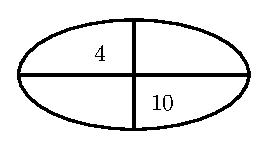
\includegraphics{figure/fig23.eps}
\end{figure}

idaralilx oMdu vAyxsavu $4\times$ matotxMdu vAyxsavu $10=40\times
.7854=31.4160$ ideV keSxVtarx Palavu.

\medskip
\begin{center}
{\bf keSxVtarxgaLa sutatxLategaLiMda keSxVtarx PalagaLanunx kANuva mAgaRvu.}
\end{center}

\begin{itemize}
\item[\rm(1)] tirxBujegaLalilx mUru bAhugaLanunx aLadu, A
yaLategaLanunx sheVrisi adhiRsi, avugaLanunx mUru sAthxnagaLalilx
baradukoMDu avugaLalilx AyA bAhugaLa aLategaLanunx kaLadu
sheVSagaLanenxlAlx parasapxravAgi guNisi A labadhxvanunx meVlakxMDa
mUru bAhugaLa vaTiTxna adhaRdiMda guNisi, A guNAkArada vagaR
mUlavanunx tegadare, tirxBuja keSxVtarxgaLa PalagaLAguvavu.

\item[\rm(2)] catuBuRjegaLidadxre, adara aLategaLanunx mADi sheVrisi,
adhaR mADi, adanunx nAlukx parxtiyAgi sAlage baradukoMDu avugaLalilx A
bAhugaLa aLategaLanunx kaLadu uLida saMKayxgaLanUnx parasapxravAgi
guNisi, A guNAkArada vagaR mUlavanunx tegadare, keSxVtarx Pala
baruvadu. 
\end{itemize}



\chapter{127neV parxkaraNa.}

\begin{center}
{\large\bf tirxBuje mitiya gaNitavu.}
\end{center}

tirxBujemitiyeMdare, tirxBujeya bAhugaLa parimitiyanUnx,
avugaLiMduMTAguva upayoVgavanUnx avu\-gaLiMda sAdhaneyAga takakx bAhu
KaMDa modalAda parimitagaLU tiLiya paDisa takakxMthAdudx idU keSxVtarx
gaNitakekx saMbaMdha paTaTxdAdxgiyeV irutatxde.


\chapter{128neV parxkaraNa}

\begin{center}
{\large\bf tirxBujeya niNaRya.}
\end{center}

\begin{verse}
kaM|| irutiha kanaRda vagaRvu| irutiha BujakoVTi yugamx
dogaRdamotatxM|| sariyAgirutira lavugaLu| varatirxBujegaLaLate
niNaRyaMgaLu shidadhxM||
\end{verse}

hAyxgeMdare,
\begin{figure}[H]
\centering
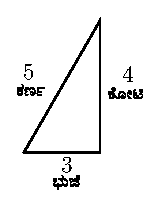
\includegraphics[scale=1.2]{figure/fig24.eps}
\end{figure}
\begin{center}
\begin{tabular}{c@{}c@{}c@{}c@{}c}
kanaR parxmANa. & & Buje parxmANa. & & koVTi parxmANa.\\
$5$ & & $4$ & & $3$\\
vagiRsalu & & \\
$25$ & = & $9$ & $+$ & $16$
\end{tabular}
\end{center}

hiVge tirxBujegaLa kanaR parxmANada vagaRvu. Buje koVTi eMba eraDu
bAhugaLa vagaRda motatxkekx sariyAgira beVku.



\chapter{129neV parxkaraNa}

\begin{center}
{\large\bf avayxkatxvAda Buje koVTi, karanx parxmANagaLanunx kaMDu hiDiya}
\vskip .3cm

{\large\bf takakxdadxnunx kuritadudx.}
\vskip .3cm

{\large\bf sUtarx 1.}
\end{center}

\begin{verse}
kaM|| piDidoMdiSaTxnu BujeyeM| doDanadanogiRsutaladanumatotxMdiSaTx||
napxDadudariMda laharisute| lodaneraDane yiSaTx kUDi
kaLadadhiRsuniV\char'366||

vi|| oMdu iSaTxvanunx BujeyeMtA kalipxsi, adanunx vagaR mADi, A
vagaRvanunx matotxMdiSaTx saMKayxdiMda BAgisi, baMda labadhxdalilx, A
yaraDaneV iSaTx saMKayxvanunx kUDi adhiRsidare, kanaR parxmANavU,
kaLadu adhiRsidare koVTi parxmANavU, Agutatxde.
\end{verse}

hAyxgaMdare, iSaTxBuje $12$ inoMdiSaTx saMKeyx $4$

vagiRsalu
\begin{align*}
144\div 4=\frac{36+4}{2} &= 20\text{~~ kanaR parx.}\\[5pt]
\frac{36-4}{2} &= 16\text{~~ koVTi parx.}
\end{align*}
\begin{center}
\begin{tabular}{cccc}
tALeV, & kanaR parx. & Buje. & koVTi.\\[4pt]
       & $20$ & $12$ & $16$
\end{tabular}
\end{center}

\begin{center}
\begin{tabular}{r@{\hspace{1cm}}c@{}l}
vagiRsalu & &\\
& $400=144+$ & $246$
\end{tabular}
\end{center}

\begin{center}
{\large\bf sUtarx 2.}
\end{center}

\begin{verse}
kaM|| piDideradiSATx saMKayxga| LoDaniridiMmamxDisaladuve
koVTiparxmANaM|| piDidiSaTxnogaRgoMDava| noDagUDalu kanaRkaLiye Buje
parimitiyuM|| 

vi|| eraDu iSaTx saMKayxgaLanunx kalipxsi, avugaLanunx guNisi
divxguNisidare, koVTi parxmANavu, matUtx A yaraDu iSaTx
saMKayxgaLanunx parasapxra vagiRsi avugaLanunx kUDisidare kanaR
parxmANavu, kaLedare Buje parxmANavu, sariyAgiruvavu.

\smallskip
\qquad\qquad iSaTx $2$\qquad matotxMdiSaTx $3$
\smallskip

eraDanU guNisi divxguNisalu $12$ ideV koVTi parxmANavu.
A iSaTxgaLanunx vagiRsalu
$$
4\qquad\qquad 9
$$
kUDisalu $13$ ideV kanaR parxmANavU.

kaLiyalu $5$ ideV bAhu parxmANavU.

tALe,
\begin{center}
\begin{tabular}{ccc}
kanaR parx. & Buje parx. & koVTi parx.\\[4pt]
$13$ & $5$ & $12$
\end{tabular}
\end{center}
pagiRsalu
$$
169=25+144
$$
\end{verse}

\medskip
\begin{center}
{\large\bf 148neV aBayx udAharaNe.}
\end{center}

\begin{itemize}
\item[\rm(1)] iSaTx Buje $4$, $8$, $15$, $16$ I parxkArakUkx
matotxMdiSaTxgaLu $1$, $2$, $3$, $4$ hiVge kalipxsiruvadakekx
sariyAguva koVTi kanaR parxmANagaLanunx kaMDu hiDi?

\item[\rm(2)] $3$, $4$ matutx $4$, $5$ matutx $5$, $6$ hiVge
kalipxtavAda iSaTxgaLige sariyAda Buje koVTi karanx parxmANagaLanunx
kaMDu hiDi?
\end{itemize}

\chapter{130neV parxkaraNa}


\begin{center}
{\large\bf iSaTx karanx parxmANakekx sariyAda Buje koVTi
parxmANagaLanunx kANavadakekx}
\vskip .3cm

{\large\bf sUtarx.}
\end{center}

\begin{verse}
kaM|| irutiha kanaRda divxguNava| niridiSaTxnu kalipxsayxdanu iSaTxda
vagaRdo|| LaritoMda kUDi BAgise| barutihudeV koVTi eMba parimita
keVLeY||

baMdA koVTiya niSaTxdo| LaMdadi guNisutatx kanaRparimANavanuM|| aMdu
kaLiyalekx BujeyuM| caMdadi barutihudu keVLu gaNakaramatadiM||

vi|| kanaRparxmANada divxguNavanunx oMdu kalipxta iSaTx saMKayxdiMda
guNisi labadhxvanunx A iSaTx saMKayxda vagaRdalilx $1$ sheVrisi
BAgisidare, A BAga labadhxveV koVTi parxmANavAguvadu. A koVTi
parxmANavanunx iSaTx saMKayxdiMda guNisi labadhxdalilx kanaR
parxmANavanunx kaLadare, Buje parxmANavAguvadu.\qquad hAyxgaMdare, 
\end{verse}

udahAraNe, karanx parxmANa $13$ idadxre, Buje koVTi parxmANagaLanunx
saqSiTxsu.
$$
\text{kanaR parx.}~ 13\qquad\quad \text{iSaTx saMKayx}~ 5 
$$

karanx parxmANa $13$ divxguNisalu $26$ idanunx iSaTx saMKayx $5$riMda
guNisalu $130$ idanunx iSaTx saMKayx $5$ra vagaRvAda $25$ralilx $1$
sheVrisidarAguva $26$riMdA BAgisalu $5$ ideV koVTi parxmANavU, idanunx
iSaTx saMKayx $5$riMda guNisalu $25$ idaralilx kanaR parxmANa, $13$
kaLiyalu $12$ ideV Buje parxmANavu.

\medskip
\begin{center}
{\large\bf 149neV aBayx udAharaNe.}
\end{center}

\begin{itemize}
\item[\rm(1)] iSaTx kanaR parxmANavu $5$, $20$, $45$, $52$ ivugaLige
sariyAda Buje koVTi parxmANagaLanunx kaMDu hiDi?
\end{itemize}



\chapter{131neV parxkaraNa}

\begin{center}
{\large\bf kanaR parxmANavU matutx BujekoVTigLa yoVgavU matutx aMtaravU}
\vskip .3cm

{\large\bf ivugaLiMda BujakoVTi parxmANagaLanunx kaMDu hiDiyuva riVti.}
\vskip .3cm

{\large\bf  sUtarx.}
\end{center}

\begin{verse}
kaM|| kanaRda vagaRva divxguNisi| niNaRyadiMduyxgamxBujeya
nogiRsikaLedaM|| naninxyiM sheVSa mUlava| muninxna yugamxdoLukUDi
kaLiyalasxmaneY|| 

vi|| kanaRparxmANada vagaRvanunx divxguNisi, adaralilx BujekoVTi
yukatxvAda parimANa saMKeyxya vagaRvanunx kaLadu, sheVSada vagaR
mUlavanunx modalina BujekoVTi yukatxvAda saMKeyalilx kUDisi
adhiRsidare, koVTi parxmANavU, kaLadu adhiRsidare Buje parxvayaNavu
Aguvadu. 
\end{verse}

udAharaNe, kanaRparxmANa $13$ BujakoVTi yukatx parxmANavu $17$ Agalu
Buje eSuTx? koVTi eSuTx?

kanaRparxmANa $13$ vagiRsalu $169$

BujakoVTigaLa yoVga $17$ vagiRsalu $289$

divxguNisalu
$$
338-289=\sqrt{49}=7
$$

\begin{longtable}{r@{\qquad\qquad}r}
\multicolumn{2}{l}{Agalu, Bu. ko. yoV. Bu. ko. yoV.}\\[3pt]
$17$ & $17$\\
$7$ & $7$\\[5pt]
\multicolumn{2}{l}{kUDi kaLiyalu}\\[2pt]
$24$ & $10$\\[5pt]
\multicolumn{2}{l}{adhiRsalu}\\[5pt]
$12$ koVTi, & $5$ Buje.\\[5pt]
\multicolumn{2}{l}{athavA}\\
karanx parxmANa & Buje ko. a.\\
$13$ & $7$\\[5pt]
\multicolumn{2}{l}{vagiRsalu}\\
$169$ & vagaR\\
$2$ & \\
\cline{1-1}
$338$ & $49$\\
$49$ & \\
$\sqrt{289}$ sheVSa\\[.5cm]
\multicolumn{2}{l}{
$=17$
$\left\{
\begin{array}{rr}
17 & 17\\
7 & 7\\
\multicolumn{2}{l}{\text{kUDi kaLadu adhiRsalu.}}\\
12 & 5
\end{array}
\right.$}
\end{longtable}

\begin{center}
{\large\bf 150neV aBayx udAharaNe.}
\end{center}

\begin{itemize}
\item[\rm(1)] karanx parxmANagaLu $25$, $50$, $26$, $65$ matutx Buje
koVTigaLa yoVgagaLu $35$, $70$, $34$, $85$ Agalu Buje koVTi
parxmANagaLanunx viMgaDisi heVLu?
\end{itemize}

\chapter{132neV parxkaraNa}

\begin{center}
{\large\bf Buje parxmANa matutx koVTi kanaRgaLa yoVga parxmANa ivugaLiMda}
\vskip .3cm

{\large\bf koVTi, kanaR parxmANagaLanunx parxteyxVkisuva mAgaRvu.}
\vskip .5cm

{\bf udAharaNe.}
\end{center}

\begin{figure}[H]
\centering
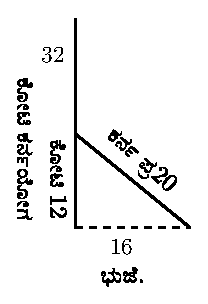
\includegraphics{figure/fig25.eps}
\end{figure}

muvavxtetxraDu aDigaLa unanxtavAda oMdu bidarina maravu GALiyiMda
murakoMDu, adara koneyu BUmige soVkuva hAge bididxtu. Agalu A
maradabuDadiMdA bididxruva vaqkaSxda koneVvarige $16$ aDigaLe
dUravidadxre, A maravu eSuTx unanxtadalilx muriVtu, matutx
muradadadxra parxmANa veSuTx?

\medskip
\begin{center}
{\large\bf sUtarx.}
\end{center}

\begin{verse}
kaM|| irutihaBujeyanonxgiRsu| taritadanAkoVTikanaRyoVgadoLahxrisu||
barutiha PalavanonxyXVgadi| pariyarituMkUDikaLedu adhiRse samaneY||

vi|| Buje parxmANavanunx vagiRsi, adanunx koVTi karanxgaLa yoVgadiMda
BAgisi, baruva labadhxvanunx A koVTi karanxgaLa yoVga saMKeyalilx kUDi
adhiRsidare karanx parxmANavu, kaLadu adhiRsidare koVTi parxmANavu
Aguvadu. 
\end{verse}

Buje athavA aMtara $16$

koVTi karanxgaLa yoVga athavA vaqkaSx parimANa $32$

vagiRsalu

\medskip

\begin{tabular}{r@{}c@{}c}
$32$ & ) & $256$\\
\cline{3-3}
 & & $8$
\end{tabular}

\begin{tabular}{rr}
\multicolumn{2}{l}{Agalu}\\
$32$ & $32$\\
$8$ & $8$\\[5pt]
\multicolumn{2}{l}{kUDi kaLiyalu}\\
$40$ & $24$\\[5pt]
\multicolumn{2}{l}{adhiRsalu}\\[2pt]
\multicolumn{1}{c}{\quad $20$ kanaR} & \multicolumn{1}{c}{\quad $12$ koVTi}
\end{tabular}

ililx A maravu $12$ aDiya unanxtadalilx murakoMDiteMtalU muradadudx
$20$ aDi parxmANaveMtalU tiLiya beVku.

\medskip
\begin{center}
{\large\bf 151neV aBayx udAharaNe.}
\end{center}

\begin{itemize}
\item[\rm(1)] Buje parxmANagaLu $5$, $15$, $15$ matutx koVTi
karanxgaLa yoVga parxmANagaLu $25$, $75$, $45$ Agiralu, avugaLalilx
koVTi karanx parxmANagaLanunx viMgaDisi heVLu?
\end{itemize}


\chapter{133neV parxkaraNa}

\begin{center}
{\large\bf Buje parxmANa matutx koVTi karanxgaLa aMtara parxmANa ivugaLiMda}
\vskip .3cm

{\large\bf koVTi karanxgaLanunx viMgaDisa takakx mAgaRvu.}
\end{center}

{\bf udAharaNe,}
\begin{figure}[H]
\centering
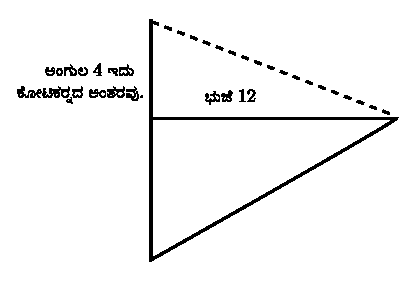
\includegraphics{figure/fig26.eps}
\end{figure}

u. oMdu saroVvaradalilx kamalavu niVrina meVle $4$ aMgulavitutx. A
kamalavanunx niVrige samanAgi eLiyalu, muMce adu idadx nALadiMda
hiDidu $12$ aMgula dUravAyitu. Agalu, A sathxLadalilx jalaparxmANa
veSuTx heVLu?

\newpage

\medskip
\begin{center}
{\bf sUtarx.}
\end{center}

\begin{verse}
kaM|| eMtiha BujeyanonxgiRsu| taMtaradiMdahxrisi koVTi
karanxgaLaMtara|| veMtihado kUDi kaLiyuta| saMtasadiMdadhiRsaduve
koVTiyukaranxM|| 

vi|| Bujeyanunx vagiRsi adanunx koVTi karanxgaLa aMtaradiMda BAgisi, A
labadhxdalilx A koVTi karanxgaLa aMtara saMKeyxyanunx kUDisi
adhiRsidare, karanx parxmANavU kaLadu adhiRsidare koVTi parxmANavU
baruvavu. 
\end{verse}

Buje parxmANa $12$

koVTi karAnxMtara $4$

vagiRsalu
\medskip

\begin{tabular}{r@{\hspace{.5cm}}r@{}c@{}c}
aMtara & $4$ & ) & $144$\\
\cline{4-4}
& & & $36$
\end{tabular}

\medskip

\begin{tabular}{rlrl}
$36$ & & $36$ &\\
$4$ & aMtara & $4$ & aMtara\\[5pt]
\multicolumn{4}{l}{kUDi kaLiyalu}\\
$40$ && $32$ &\\[5pt]
\multicolumn{2}{l}{adhiRsalu}\\[2pt]
$20$ & karanx parx. & $16$ & idu koVTi athavA jala parxmANavu.
\end{tabular}

\begin{center}
{\large\bf 152neV aBayx udAharaNe.}
\end{center}

\begin{itemize}
\item[\rm(1)] Buje parxmANagaLu $5$, $15$, $15$ koVTi karAnxMtara
parxmANagaLu $1$, $3$, $5$ Agalu, koVTi karanxgaLanunx parxteyxVkisi
heVLu? 
\end{itemize}


\chapter{134neV parxkaraNa}

\begin{center}
{\large\bf koVTi parxmANa matutx Buje karanxgaLa yoVga parxmANa ivugaLiMda}
\vskip .3cm

{\large\bf Buje karanxgaLanunx parxteyxVkisuva mAragxvu.}
\end{center}

\begin{figure}[H]
\centering
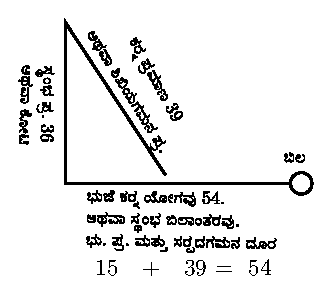
\includegraphics{figure/fig27.eps}
\end{figure}

u. $36$ aDi unanxtavAda oMdu kaMBada meVle oMdu navilu kUtitutx. A
kaMBada buDadiMda $54$ aDi dUradalilx oMdu biladalilx sarapxvitutx,
Agalu A sarapxvu kaMBada buDada mAragxvanunx kuritu hoVgutitxralAgi A
navilu tAnidadx sathxLadiMda karanx sUtarx mAragxvAgi hAri baMdu A
sarapxvanunx hiDakoMDitu, Aga noVDalAgi A sarapx shiKigaLa gamana
dUravU oMdeV samanAgitutx. Adare A navilina gamana dUravanUnx sarapx
shikikxda sathxLakUkx kaMBakUkx yiruva aMtaravanunx eSATxgutetxMdu
tiLidu heVLu? 

\medskip
\begin{center}
{\bf sUtarx.}
\end{center}

\begin{verse}
kaM|| irutiha koVTiya nogiRsu| taritadanaM bAhukaranx
yoVgadoLahxrisu|| barutiha Pala\-vAyoVgadi| sarigUDisi kaLaduadhaR
mADalasxmaneY||

vi|| koVTi parxmANavanunx varigxsi, adanunx Buje karanxgaLa yoVga
saMKeyiMda BAgisi, A labadhxvanunx A Buje karanxgaLa yoVga saMKeyalilx
kUDisi adhiRsidare, karanx parxmANavu, kaLadu adhiRsidare, Buje
parxmANavu, Agutatxde.
\end{verse}

koVTi athavA sathxMBa parxmANavu $36$

Buje karanxgaLayoVga athavA kaMBadiMda biladavarige iruva dUra $54$

varigxsalu
\medskip

\begin{tabular}{r@{}c@{}c}
$54$ & ) & $1296$\\
\cline{3-3}
 & & $24$
\end{tabular}

\medskip

\begin{tabular}{rlrl}
\multicolumn{4}{l}{Agalu}\\
\multicolumn{4}{l}{\quad Buje karanxgaLa yoVga}\\
$54$ & & $54$ &\\
$24$ & BAga labadhx & $24$ &\\[4pt]
\multicolumn{4}{l}{\quad kUDi kaLiyalu}\\[2pt]
$78$ &  & $30$ &\\
\multicolumn{4}{l}{\quad adhiRsalu}\\[2pt]
$39$ & karanx & $15$ & Buje.
\end{tabular}

\begin{itemize}
\item[sU||] ililx $39$ karanx parxmANa athavA navilina gamana
dUraveMtalU $15$ Buje parxmANa athavA sathxMBakUkx sarapx sikikxda
sathxLakUkx iruva dUraveMtalU idanunx A yoVga parxmANa $54$ralilx
kaLiyalu $39$ idu sarapx gamana parxmANaveMtalU tiLiya beVku.
\end{itemize}

\begin{center}
{\large\bf 135neV aBayx udAharaNe.}
\end{center}

\begin{itemize}
\item[\rm(1)] koVTiya parxmANagaLu $9$, $12$, $20$ Buje karanxgaLa
yoVga parimANagaLu $27$, $18$, $40$ Agalu, Buje karanx
parxmANagaLanunx viMgaDisi heVLu?
\end{itemize}


\chapter{135neV parxkaraNa}

\begin{center}
{\large\bf Buje parxmANa matutx koVTiya KaMDavU ivugaLa AdhAradiMda uLida}
\vskip .3cm

{\large\bf koVTi parxmANa matutx karanxparxmANagaLanunx kANuva mAgaRvu.}
\end{center}

\begin{figure}[H]
\centering
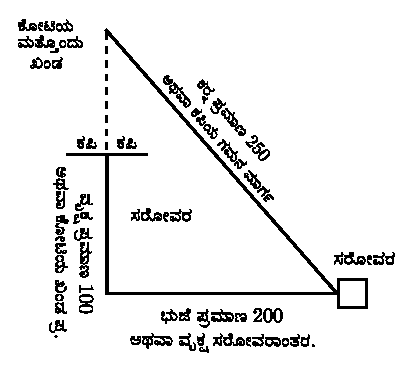
\includegraphics{figure/fig28.eps}
\end{figure}

udAharaNe, oMdu teMgina vaqkaSxvu $100$ aDi unanxtavAgitutx. adara
buDadiMda $200$ aDi dUradalilx oMdu saroVvaravitutx. Agalu, A
vaqkaSxda meVle kUtidadx, eraDu kapigaLalilx oMdu A vaqkaSxdiMda
yiLadu saroVvarakekx niVru kuDiyuvadakekx hoVyitu. matotxMdu A
vaqkaSxdiMda kelavu aDi meVlakekx negedu alilxMdA karanx sUtarx
mAgaRvAgi A saroVvarakekx hAritu. Aga noVDalAgi averaDara gamana
dUravu oMdeV samanAgidadxvu. Adare A eraDaneV kapi hArida
unanxtaveSuTx? matutx alilxMdA saroVvaradavarige hArida dUraveSuTx
heVLu?

\begin{center}
{\large\bf sUtarx.}
\end{center}

\begin{verse}
kaM|| BujekoVTi KaMDa guNisuta| nijadiMdA koVTi KaMDa divxguNadi
kUDida|| BujeyiMdhahxri\-salabxruvadu| rujuvAgiha koVTi KaMDa
gaNakaramatadiM||

vi|| BujeyanUnx koVTi KaMDa parxmANavanUnx guNisi, A labadhxvanunx
(koVTiya KaMDada divxguNadalilx Buje parxmANavanunx sheVrisidare Aguva
saMKayxdiMda) BAgisu baruva labadhxveV uLida koVTi KaMDa
parxmANavAgiruvadu. 
\end{verse}

riVtiyu, Buje parxmANa $200\times 100$ koVTiya KaMDa
$=\underline{20000}$ idanunx koVTiya KaMDa $100$ divxguNa $200+200$
Buje parx. $=400$

BAgisalu $50$ ideV koVTiya matotxMdu KaMDa parxmANavu.

\begin{itemize}
\item[sU||] idaralilx vaqkaSx parxmANa $100$nunx koVTiya KaMDaveMtalU,
vaqkaSxkUkx saroVvarakUkx iruva dUra $200$nunx Buje parxmANaveMtalU
meVlakekx hAridaMthA $50$ koVTiya matotxMdu KaMDaveMtalU A koVTiya
koneyiMdA saroVvaradavarige hAri baMda gamana parxmANa $250$nunx
karanx parxmANaveMtalU tiLiya beVku.
\end{itemize}

\begin{center}
{\large\bf 154neV aBayx udAharaNe.}
\end{center}

\begin{itemize}
\item[\rm(1)] Buje parxmANa $120$ matutx koVTiya KaMDa parxmANavu $40$
aDigaLidadxre, uLida koVTi parxmANa matUtx karanx parxmANagaLeSeTxMdu
tiLidu heVLu?
\end{itemize}



\chapter{136neV parxkaraNa}

\begin{center}
{\large\bf eraDu koVTi parxmANagaLu matutx averaDara BujegaLa yoVga parxmANavu}
\vskip .3cm

{\large\bf ivugaLiMda avugaLa parxteyxVka parxteyxVkavAda Buje karanx
parxmANagaLanunx} 
\vskip .3cm

{\large\bf kANuva mAgaRvu.}
\end{center}

\begin{figure}[H]
\centering
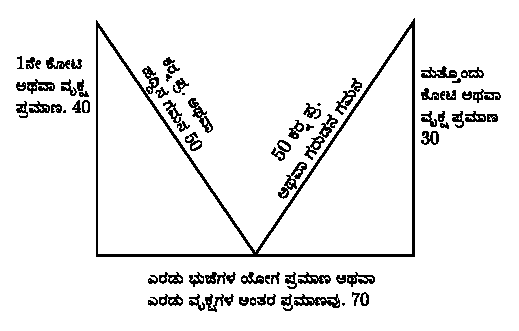
\includegraphics{figure/fig29.eps}
\end{figure}

parxshenxV. $40$ matutx $30$ aDigaLa unanxtavAda eraDu vaqkaSxgaLa
madhayxdalilx $70$ aDi aMtaragaLuMTu. A eraDu vaqkaSxgaLalilx oMdara
meVle hadudx matotxMdara meVle garuDa hiVge eraDu pakiSxgaLu
kUtidadxvu. Aga oMdu vaqkaSx buDadiMda oMdu sapaRvu matotxMdu
vaqkaSxda kaDege hoVgutAtx yitutx. Aga adanunx A eraDu pakiSxgaLU
kaMDu avugaLu kUtidadx sathxLadiMda karanx sUtarx gatiyAgi hAri baMdu
A sapaRvanunx hiDakoMDavu. Aga A veraDara gamana mAgaRvu eMdeV
samanAgi yidadxvu. Adare averaDu pakiSxgaLa gamana parxmANagaLanUnx
matutx sapaR shikikxdaMthA sathxLakUkx A eraDu vaqkaSxgaLigU iruva
BUje parxmANavanUnx tiLadu heVLu?

\medskip
\begin{center}
{\large\bf sUtarx.}
\end{center}

\begin{verse}
kaM|| eraDu BujeyoVgadogaRdi| eraDuM koVTigaLavagaRdoLa goMdanukU||
DiradelekaLi matotxMdanu| sarikoVTiga LeraDaroyxVga
doLagadanahxriseY||

barutihudeV bAhuKaMDaga| LaritavanuM koVTigaLanu| vagiRsikUDu||
tatxradavagaLa mUlagANalf sariyAguva daduvekaranx parimANagaLU||

vi|| eraDu BujegaLa yoVgada vagaRdalilx oMdu koVTiya vagaRvanunx
sheVrisi, A vaTiTxnalilx matotxMdu koVTiya vagaRvanunx kaLadu
uLidadadxnunx (A eraDu koVTi parxmANagaLU matutx eraDu BujegaLa yoVga
parxmANa) ivugaLa yoVgadiMda BAgisidare, baruva BAga labadhxveV oMdu
bAhuvina parxmANavAgiruvadu, adanunx A eraDu bAhugaLa yoVga
parxmANadalilx kaLadare, matotxMdu bAhu parxmANavAguvadu. taruvAya,
AyAya bAhugaLu matutx koVTi parxmANagaLanunx vagiRsi sheVrisi, A vaTi
na vagaR mUlagaLanunx tegadare, karanx parxmANagaLu athavA pakiSxgaLa
gamana parxmANagaLu baruvavu.
\end{verse}

\begin{figure}[H]
\centering
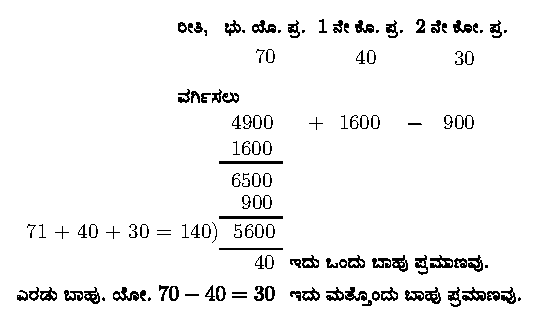
\includegraphics[scale=1.1]{figure/fig30.eps}
\end{figure}

\smallskip

\begin{tabular}{ccccccc}
\multicolumn{7}{l}{Agalu,}\\
koV. & & bA. & & koV. & & bA.\\[2pt]
$40$ & & $30$ & & $30$ & & $40$\\[5pt]
\multicolumn{7}{l}{vagiRsalu}\\
$1600$ & + & $900$, & & $900$ & + & $1600$\\[5pt]
\multicolumn{7}{l}{sheVrisalu}\\
$2500$ & & & & & & $2500$\\[5pt]
\multicolumn{7}{l}{vagaR mUlavanunx mADalu}\\
$50$ & & & & & & $50$\\[5pt]
\end{tabular}

ivugaLeV kanaR parxmANagaLu athavA pakiSxgaLa gamana parxmANagaLU.

\smallskip
\begin{center}
{\large\bf 155neV aBayx udAharaNe.}
\end{center}

\begin{itemize}
\item[\rm(1)] eraDu tirxkoVNada BujegaLa yoVga $49$ matutx oMdara
koVTi $28$ matotxMdara koVTi $21$ aDigaLa parxmANagaLidadxre, A
eraDara bAhu kanaR parxmANagaLanunx viMgaDisi heVLu?
\end{itemize}



\chapter{136neV parxkaraNa}

\begin{center}
{\large\bf oMdu tirxkoVNA kaqtiya bAhu parxmANagaLiMda adara laMba
parxmANavanUnx}
\vskip .3cm

{\large\bf matutx laMba reVKeya Ace Icegiruva pAda parimANa}\\
\vskip .3cm

{\large\bf athavA AbAdhegaLanUnx kaMDu hiDiyuva mAgaRvu.}
\end{center}

\begin{figure}[H]
\centering
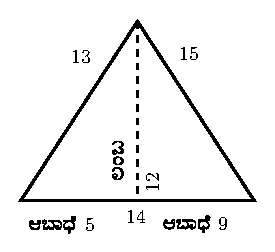
\includegraphics{figure/fig31.eps}
\end{figure}

udAharaNe, I tirxkoVNada bAhugaLu $13$, $14$, $15$ aDi
parxmANagaLidadxre A tirxkoVNada laMba athavA unanxtaveSuTx matutx A
laMboVBaya pashavxRda AbAdhegaLeSuTx heVLu?

\medskip
\begin{center}
{\large\bf sUtarx.}
\end{center}

\begin{verse}
kaM|| BujeyoV bAhu motatxva| Buje eraDara sheVSadiMdaliriyutatxdanaM||
Buje pAdadoLahxrisi baMduda| nijapAdadoLaLidu gUDiyadhiRse KaMDaM||

baMdiha KaMDagaLogiRsu| taMdadaroLagadara bAhu vagaRva kaLadA| daMdava
mUlaM gANalu baMdapudeY laMbavAga gaNakaramatadiM||

vi|| pAdoVpari yiruva bAhugaLa yoVgavanunx A bAhugaLa aMtaradiMda
guNisi labadhxvanunx pAda parxmANadiMda BAgisi, baruva labadhxvanunx A
pAda parxmANadalilx kUDisi adhiRsidare, doDaDx tirxkoVNada pAda athavA
AbAdheyU kaLadu adhiRsidare, cikakx tirxkoVNada pAda athavA A bAdheyU
barutatxve. taruvAya, AyAya AbAdhe matutx bAhugaLanunx vagiRsi kaLadu
sheVSada vagaR mUlavanunx tegadare, laMba parxmANagaLu barutatxve. 
\end{verse}

\medskip

\begin{tabular}{rrcr}
riVti, Buje & $13+15$ & = & $28$\\
            & $15-13$ & = & $2$\\
\cline{4-4}
 & pAda~~ $14)$ && $56$\\
\cline{4-4}
& & & $4$
\end{tabular}

\medskip

\begin{tabular}{rr}
\multicolumn{2}{l}{pAdavu}\\[2pt]
$14$ & $14$\\
$4$ & $4$\\[5pt]
\multicolumn{2}{l}{kUDi kaLiyalu}\\[2pt]
$18$ & $10$\\[5pt]
\multicolumn{2}{l}{adhiRsalu}\\[2pt]
$9$ & $5$
\end{tabular}

Agalu, Buje $15$\qquad $9$ AbAdhe

vagiRsalu\quad $225-81$

kaLiyalu\quad $144$

vagaR mUla $12$ ideV laMba parxmANavu.

Buje 13\qquad AbAdhe 5

vagiRsalu\quad $169-25$

kaLiyalu\quad $144$

vagaR mUla $12$ idU laMba parxmANavu.


\medskip

\begin{center}
{\large\bf 156neV aBayx udAharaNe.}
\end{center}

\begin{itemize}
\item[\rm(1)] oMdu tirxkoVNada pAdoVpari bAhugaLa parxmANavu $39$,
$45$ matutx adara pAda parxmANavu $42$ idadxre, Adara laMbana matutx
AbAdhegaLeSuTx heVLu?
\end{itemize}



\chapter{138neV parxkaraNa}


\begin{figure}[H]
\centering
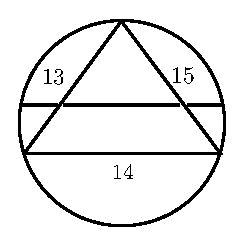
\includegraphics{figure/fig32.eps}
\end{figure}

tirxBujeya bAhayxdalilx A tirxBujeya koVNagaLu paridhige
sapxshaRvAguvaMteV vaqtatxvanunx baradare A vaqtatx parimANa viSeTxMdu
kaMDu hiDiyuva mAgaRvu.

udAharaNe, $13$, $14$, $15$ aDigaLa parxmANavuLaLx tirx BujAdabxhi
barada vaqtatx parxmANa veSuTx heVLu?

\medskip
\begin{center}
{\large\bf sUtarx.}
\end{center}

\begin{verse}
kaM|| cikakx bAhugaLa vagaRva| nakakxradiMsheVrisayxdara
mUlavategadU|| mikakx paribAhu sheVrisi Gakakxneya\-dhaRvanu
mADaladuvAsayxvukeVLi||

vi|| cikakx bAhugaLa vagaRgaLa yoVgada vagaR mUlavanunx tegadu A
mUladalilx uLida doDaDx bAhu parxmANavanunx sheVrisi athaRvanunx,
mADidare, vAyxsa parxmANa biruvadu.
\end{verse}

\medskip

\begin{tabular}{rr}
\multicolumn{2}{l}{riVti,}\\
$13$, & $14$\\[5pt]
\multicolumn{2}{l}{vagiRvu}\\
$169$ & $196$\\[5pt]
\multicolumn{2}{l}{yoVgavu}\\
 & $365$\\[5pt]
\multicolumn{2}{l}{adara mUlavu.}\\
 & $19.1$
\end{tabular}

\medskip

$19.1$ mUla\qquad $15$ vikakxpiri bAhu

sheVrisalu $34.1$

adhiRsalu $17.05$

ideV vAyxsa parxmANavu. idakekx muMce heVLiruva parxkArakekx
paridhiyanunx sAdhisi koLaLx beVku.

\medskip
\begin{center}
{\large\bf 157neV aBayx udAharaNe.}
\end{center}

\begin{itemize}
\item[\rm(1)] $5$, $12$, $13$, matutx $12$, $9$, $15$ I riVti bAhu
parimANagaLuLaLx tirxBujegaLa bAhayxdalilx barada vaqtatxgaLa
parxmANagaLanunx heVLu?
\end{itemize}

\chapter{139neV parxkaraNa}

catuBuRjegaLa bAhayxdalilx barada vaqtatx parxmANagaLanunx kaMDu
hiDiyuva mAgaRvu?
\begin{figure}[H]
\centering
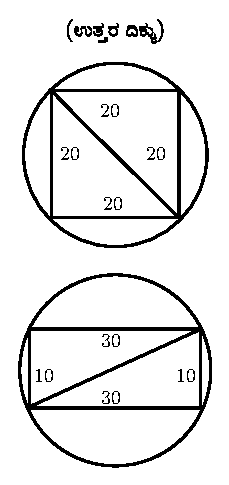
\includegraphics{figure/fig33.eps}
\end{figure}

u. nAlukx bAhugaLU $20$ aDigaLa parxmANagaLuLaLx cacwcxkA kaqtiya
bAhayxdalilx adara koVNaLelAlx paridhige vAyxpisuvaMteyU, matutx
ililx kANisuva inonxMdu Ayaka keSxVtarxda bAhayxdalUlx barada eraDu
vaqtatx parxmANagaLanunx kaMDu hiDi?

\medskip
\begin{center}
{\large\bf sUtarx.}
\end{center}

\begin{verse}
kaM|| utatxra pUvaRda BujegaLa| parxteyxVkadoLogaRgoMDu kUDuta mUlaM||
bitatxradi kANaladuvaM ititxha vaqtatxkekx vAyxsa tirxBujada kaNaRM||

vi|| utatxra pUvaR bAhugaLanUnx parxtayx parxteyxVkavAgi vagaRgaLanunx
mADi, A eraDu vagaR saMKayxgaLanunx kUDisi adara vagaR mUlavanunx
tegedare, vAyxsa parxmANa baruvadu. I vAyxsa parxmANavu A
catuBuRjegaLa kanaR parxmANakekx sariyAgiruvadu.
\end{verse}

\medskip

($1$neVdu)
\smallskip

\begin{tabular}{cc}
u. & pU.\\
$20$ & $20$
\end{tabular}

vagiRsalu\qquad $400+400$

sheVrisalu\qquad $800$

mUlavu\qquad $28.28$ 

ideV vAyxsa parxmANavu. matutx, kanaR parxmANavu Agiruvadu.

\medskip

($2$neVdu)
\smallskip

\begin{tabular}{cc}
utatxra & pUvaR\\
$30$ & $10$\\[5pt]
\multicolumn{2}{l}{vagiRsalu}\\
$900$ & $100$
\end{tabular}

kUDisalu\qquad $1000$

vagaR mUlavu\qquad $31.62$

ideV vAyxsa parxmANavu, matutx karanx parxmANavAgiruvadu.

\medskip

\begin{center}
{\large\bf 158neV aBayx udAharaNe.}
\end{center}

\begin{itemize}
\item[\rm(1)] utatxra pUvaRda bAhugaLu $9$, $16$ matutx dakiSxNa
pashicxma bAhugaLu $36$, $25$ aDigaLuLaLx catuBuRjAdabxhiV barada
vaqtatx parxmANaveSATxgutetx, heVLu.
\end{itemize}


\chapter{140neV parxkaraNa}

\begin{center}
{\large\bf catuBuRja, tirxBuja parxmANagaLiMda adara bAhugaLu
paridhige sapxshaR}
\vskip .3cm

{\large\bf vAguvaMteV baradaMthA vaqtatx parxmANavanunx kaMDu hiDiyuva
mAgaRvu.}
\end{center}

udAharaNe, $13$, $14$, $15$ aDigaLa bAhu parxmANagaLuLaLx
tirxBujAMtagaRtavAda vaqtatx parxmANaveSuTx, heVLu?
\begin{figure}[H]
\centering
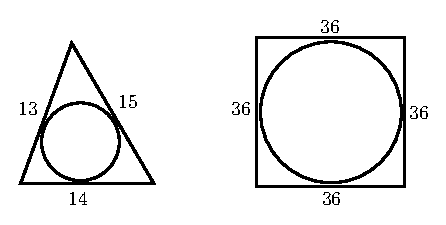
\includegraphics{figure/fig34.eps}
\end{figure}

\begin{center}
{\large\bf sUtarx.}
\end{center}

\begin{verse}
kaM|| irutiha tirxBujada Palava| nanxritA tirxBujegaLayoVga
dadhaRdoLahxrisa|| labxrutihudu vAyxsa \hbox{dadhaRvu|} aritadanaM
peVLugaNaka paramAshacxrayxM||

Palacatura keSxVtarx Bujeyada| nolaviMdA bAhucatura yoVgAdhaRdoLo||
nilade harisalekx baruvadu| neleyAgiha vAyxsadadhaR gaNakaramatadiM||

vi|| tirxBujada keSxVtarx Palavanunx adara tirxbAhugaLa yoVgAdhaRdiMda
BAgisidare, baruva labadhxveV vAyxsAdhaR
parxmANavAgiruvadu. catuBuRjada keSxVtarx Palavanunx A catubARhugaLa
yoVgAdhaR\-diMda BAgisidare baruva labadhxveV vAyxsAdhaRvAgiruvadu. 
\end{verse}

riVti, meVlina tirxBujeya laMbavu $12$nunx sAdhisi keSxVtarx
Palavanunx mADalu $84$ idanunx adara bAhugaLAda $13+14+15=42$ idara
adhaRvu $21$ idariMda BAgisalu $4$ ideV vAyxsAdhaR parxmANavu.

matutx meVlina catuBuRja keSxVtarx Palavanunx A catubARhugaLa
yoVgAdhaRdiMda BAgisidare, baruva labadhxvu vAyxsAdhaRvAgiruvadu.

riVti, meVlina catuBuRjeya keSxVtarx Palavu $36^{2}=1296$ idanunx
$36+36=36+36=144$ adara adhaRvu $72$ idariMda BAgisalu $18$ ideV
vAyxsAdhaR parxmANavAgiruvadu.

\medskip
\begin{center}
{\large\bf 159neV aBayx udAharaNe.}
\end{center}

\begin{itemize}
\item[\rm(1)] $36$, $48$, $60$ aDigaLa parxmANavuLaLx tirxBujeyavaLagU
matutx utatxra pUvaR bAhugaLu $36$, $36$ pashicxma dakiSxNa bAhugaLu
$24$, $24$ aDigaLuLaLx catuBuRjadoLagU barada vaqtatx parxmANagaLeSuTx?
\end{itemize}



\chapter{141neV parxkaraNa}

\begin{center}
{\large\bf vaqtatx keSxVtArxMtagaRtavAda mUrAdiyAda sama bAhugaLuLaLx}
\vskip .3cm

{\large\bf keSxVtarxgaLa bAhu parxmANagaLanunx athavA jAyx parxmANaga}
\vskip .3cm

{\large\bf Lanunx kaMDu hiDiyuva mAgaRvu.}
\end{center}

\medskip
\begin{center}
{\large\bf akaSxra sAjecnxya sUtarxvu.}
\end{center}

\begin{verse}
kaM|| ganaLabanaka tirxBujakukxM| gaNada GajA catura
Bujake. GaDashanadheYdU| anaKaKata mAru BujakaM|
maNanaKashAsapatxBujege KaThadhaNaDaSaTxM||

iMtu dhaqvAMkigaLariyuta | leMtihadA vaqtatxvAyxsa gaLaniriyutatxda||
naMtu naKanaKaGaTadoLuM| aMtakukxM harisipeVLu bAhu parxmANaM||

vi|| $103903$ mUru bAhuvigU, $84853$ catuBuRjegaLigU, $70534$
paMcaBujegaLigU, $60000$ Aru BujegaLigU, $52055$ ELu BujegaLigU,
$45922$ eMTu BujegaLigU, I kalipxtavAda dhaqvAMkigaLanunx AyA
vaqtatxda vAyxsa parxmANagaLiMda guNasi, A labadhxgaLanunx $120000$
diMda BAgisidare, baruva labadhxveV AyA vaqtatxgaLa bAhugaLu athavA
aSaTxSuTx jAyx parxmANagaLAgiruvavu.
\end{verse}

\begin{figure}[H]
\centering
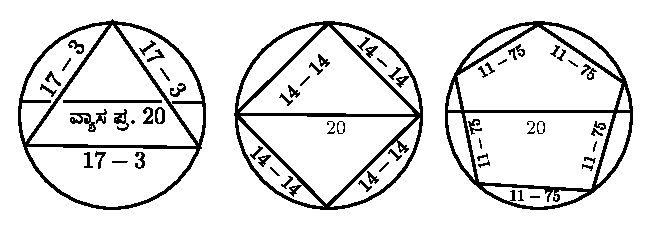
\includegraphics{figure/fig35.eps}
\end{figure}

\begin{itemize}
\item[\rm(1)] mUru bAhugaLige dhaqvAMki $103903\times 20$ vAyxsa $\div
120000=17.3$ 

\item[\rm(2)] nAlukx bahugaLige daqvAMki $84853\times 20$ vAyxsa $\div
120000=14.14$ 

\item[\rm(3)] aidu bAhugaLige dhaqvAMki $70534\times 20$ vAyxsa $\div
120000=11.75$ 
\end{itemize}

\medskip

\begin{center}
{\large\bf 160neV aBayx udAharaNe.}
\end{center}

\begin{itemize}
\item[\rm(1)] $100$ aDi vAyxsa uLaLx vaqtatxgaLalilx baradaMthA $6$,
$7$, $8$ bAhugaLuLaLx keSxVtarxgaLa bAhu parxmANagaLeSuTx?
\end{itemize}


\chapter{142neV parxkaraNa}

\begin{center}
{\large\bf vaqtatx davxyada saMyoVga sAthxnadalilx AyAya vaqtatxgaLa}
\vskip .3cm

{\large\bf sharAnayanagaLanunx kaMDu hiDiyuva mAgaRvu.}
\end{center}

\begin{figure}[H]
\centering
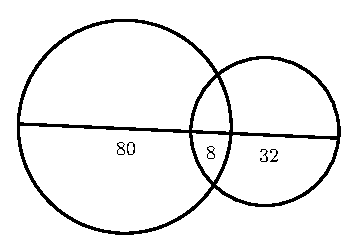
\includegraphics{figure/fig36.eps}
\end{figure}

u. $80$ aDi vAyxsavuLaLx doDaDx vaqtatxvanunx $32$ aDi vAyxsavuLaLx
cikakx vaqtatxvu sapxshaRvanunx mADiruva sathxLada madhayxdalilx $8$
aDi parxmANa gArxsavAgidhe. Agalu doDaDx vaqtatxdalilx cikakx vaqtatx
gArxsa matutx cikakx vaqtatxdalilx doDaDx vaqtatxda gArxsa I eraDu
parxmANagaLeSiTxra bahudu, heVLu?

\medskip

\begin{center}
{\large\bf sUtarx.}
\end{center}

\begin{verse}
kaM|| vaqtatxda vAyxsadigArxsava| notatxrisutasheVSa yoVgavanu
mADutatxM|| vaqtatxda sheVSava gArxsado| Letitxriduda BAgigANaladu
sharamitiyU|| 

vi|| vaqtatxgaLa vAyxsa parxmANagaLalilx gArxsa parxmANavanunx kaLadu
sheVSagaLanunx sheVrisi, adariMda A sheVSAMkigaLanunx gArxsa
parxmANadiMda guNisidaMthA labadhxgaLanunx BAgisidare, baruva
labadhxgaLeV shara parxmANagaLAgiruvavu.
\end{verse}

$80$\qquad $8$ gArxna parx.

kaLiyalu $72$\qquad $8$ gArxsa parx.

guNisalu $96)~ 576$\qquad $6$ shara parx.

idu cikakx vaqtatxdudx.

$32$\qquad $8$ gArxsa parxmANa.

$24$ kUDisalu $96$\qquad $8$ gArxsa parx.

$96)$~ $192$\qquad $2$ shara parxmANa.

idu doDaDx vaqtatxdudx. 

\medskip

\begin{center}
{\large\bf 160neV aBayx udAharaNe.}
\end{center}

\begin{itemize}
\item[\rm(1)] $200$ matutx $100$ aDigaLa vAyxsagaLuLaLx eraDu
vaqtatxgaLa saMyoVga sAthxnadalilx $50$ aDigaLa parxmANa
gArxsa\-vAgidadxre, A eraDu vaqtatxgaLa gArxsa parxmANagaLeSiTxra
bahudu?
\end{itemize}


\chapter{143neV parxkaraNa}

\begin{center}
{\large\bf vaqtatxdalilx vAyxsa matutx shara parxmANadiMda jAyx parxmANagaLanunx}
\vskip .3cm

{\large\bf athavA vAyxsa matutx jAyx parxmANagaLiMda shara parxmA}
\vskip .3cm

{\large\bf NagaLanunx kANuva mAgaRvu.}
\end{center}

\begin{verse}
shara parxmANakekx sUtarx|| jAyx vAyxsada yoVgavanA| jAyx
vAyxsAMtaradoLiridu mUlavategiyu|| tAtx vAyxsadi kaLadadhiRsa|
lAvAgadu sharada mitiyu gaNakaramatadiM||

jAyx parxmANakekx sUtarx|| eMtiha sharavAyxsa daMtara| vaMtAtxshara
doLage guNisi mUlava tegiyu| tatxMtada divxguNise jAyxmiti|
baMtenipudu keVLu gaNaka paramAshacxrayxM||
\end{verse}

\begin{description}
\item[\textmd{vi||} \rm(1)]
jAyx vAyxsagaLa yoVgavanunx A jAyx vAyxsagaLa aMtaradiMda guNisi vagaR
mUlavanunx tegadu A mUlavanunx vAyxsadalilx kaLadu adhiRsidare, shara
parxmANa baruvadu.

\item[\rm(2)] vAyxsa sharAMtaravanunx sharadiMda guNisi vagaR
mUlavanunx tegadu A mUlavanunx divxguNisidare, jAyx parimitiyAguvadu. 
\end{description}

\begin{figure}[H]
\centering
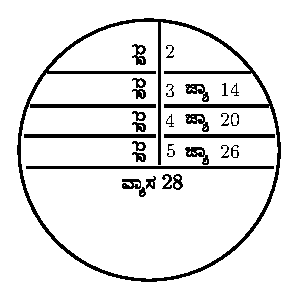
\includegraphics{figure/fig37.eps}
\end{figure}

\begin{center}
{\bf riVti.}
\end{center}

u. {\rm(1)} vAyxsa $28$ shara $2$ ivugaLiMda jAyx parxmANavanunx
matutx vAyxsa $28$ jAyx $14$ ivugaLiMda shara parxmANavanUnx kaMDu
hiDi?

\medskip

\begin{tabular}{c@{\qquad}c}
vAyxsa. & shara.\\
$28$ & $2$
\end{tabular}
\smallskip

kaLiyalu $26$

adanunx shara $2$ riMda guNisalu $52$

vagaR mUlavu $7$

divxguNisalu $14$\quad ideV jAyx parxmANavu

\medskip

\begin{tabular}{c@{\qquad}c}
vAyxsa. & jAyx.\\[2pt]
$28$ & $14$
\end{tabular}
\smallskip

yoVgavu $42$

aMtara $14$ riMda guNisalu $588$

vagaR mUlavu $24$ Agalu vAyxsa $28-24$ mUla $=4$ idanunx adhiRsalu $2$
ideV shara parxmANavU.

idaraMteyeV kaDameVdanunx Uhisa bahudu.

\medskip

\begin{center}
{\bf 161neV aBayx udAharaNe.}
\end{center}

\begin{itemize}
\item[\rm(1)] vAyxsa $28$, $28$ matutx shara parxmANagaLu $5$, $9$
ivugaLiMda jAyx parxmANagaLanUnx A baMdaMthA jAyx parxmANagaLU matutx
vAyxsa $28$, $28$ ivugaLiMda shara parxmANagaLanUnx kaMDu hiDi?
\end{itemize}


\chapter{144neV parxkaraNa}


\begin{center}
{\large\bf (\boldmath$1$)}
\vskip .3cm

{\large\bf vaqtatxda jAyx parxmANa matutx (jAyxdhaRkekx yaLiyalapxTaTx
shara parxmANakUkx}
\vskip .2cm

{\large\bf jAyxdhaR parxmANakUkx iruva karanx parxmANavU) ivugaLa AdhAra}
\vskip .2cm

{\large\bf diMda jAyxdiMda CeVdisalapxTaTx vaqtatx paridhi parxmA}
\vskip .2cm

{\large\bf Navanunx sAdhisa takakx mAragxvu.}
\end{center}

\medskip

\begin{center}
{\bf sUtarx.}
\end{center}

jAyxdhaR parxmANa $12$ shara parx. $8$ iveraDU tirxBujeya
bAhugaLAgiruvadadxriMda ivugaLiMda karanx parxmANavanunx sAdhisalu
$12$ra vagaRvu $144$.
\begin{figure}[H]
\centering
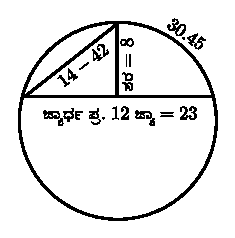
\includegraphics{figure/fig38.eps}
\end{figure}

$8$ra vagaRvu $21$

$\sqrt{208}=14.42$ karanx parxmANavu.

Iga karanx parxmANa $14.42$

jAyxdhaR parx. $12$

ivugaLiMdA aKaMDada paridhiyanunx sAdhisuvadakekx sUtarx.

\begin{verse}
kaM|| sharajAyxraLa matakaranxva| niridoTiTx roLada roLaLiyu
jAyxparimANaM|| barutiha labadhxva mUraro| Laridharisalf vaqtatxKaMDa
paridhiparxmANaM|| 

vi|| shara jAyxdhaR parxmANagaLige aBimuKavAgiruva karanx
parxmANavanunx $8$riMda guNisi, A labadhxdalilx jAyx parxmANavanunx
kaLedu uLida labadhxvanunx $3$riMdA BAgisidare, baruva labadhxveV
paridhiya BAgada aLateyAgiruvadu. hAyxgeMdare, meVlina Akaqtiyalilx
jAyx parxmANa $824$ matutx karanx parxmANa $14.42$ irutatxdeyaSeTx,
adara paridhi KaMDa parxmANa eSeTxMdare,
\end{verse}

karanx parxmANa $14.42\times 8=115.36-24$

jAyx parx. $=91.36\div 3=30.45$ idu paridhiya KaMDa parxmANa.

\medskip

\begin{center}
{\bf $2$neV riVti.}
\end{center}

vaqtatxda KaMDada saleyanunx kANuva mAragxvu.
\begin{figure}[H]
\centering
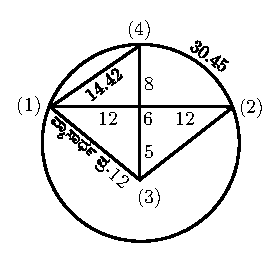
\includegraphics{figure/fig39.eps}
\end{figure}

idaralilx $1$ - $2$ yeMba jAyx parxmANavu $24$ matutx $1$ - $3$ yeMba
vAyxsAdhaR parxmANavu $13$ Adare $1$ - $4$ - $2$ - $1$ eMba KaMDada
sale eSuTx? matutx $1$ - $5$ - $2$ - $1$ eMba doDaDx KaMDada sale
eSuTx aMdare,

\begin{center}
{\bf vidhi.}
\end{center}

kaM|| vaqtatxda KaMDada paridhiya| matatxdhiRsu tadanuvAyxsa
dadhaRdoLiridaM|| vaqtatxda keVMdarxdi jAyxvari gititxha tirxBuje
parxmANa kaLiyalf PalaveY||

\begin{verse}
vi|| vaqtatxda KaMDada paridhiyanunx adhiRsi labadhxvanunx
vAyxsAdhaRdiMda guNisi, adaralilx vaqtatxda keVMdarxdiMda jAyx varige
Aguva tirxBuje parxmANada saleyanunx kaLadare, uLiyuvadeV vaqtatxda
KaMDada PalavAgiruvadu.

riVti, idaralilx vaqtatxda keVMdarxvAda $3$ iruva sathxLadiMda $4$ra
varige yaLadiruva $3$ - $4$ eMba saraLa reVKeyu $6$neV sAthxnadalilx
jAyx reVKeyanunx adhiRsutatxde, AdadxriMda $1$ - $6$ = $12$ aDi
Ayitu. matutx, $1$ - $6$ = $12$ matutx $1$ - $3$ = $13$ Agalu, hiMdina
tirxkoVNa maDiV parxkArakekx $3$ - $6$ = $5$ Ayitu. Agalu, hiMde
sAdhisiruva meVrige cikakx KaMDada paridhi parxmANavu $80.45$
adhiRsalu $15.275\times 13$ vAyxsAdhaR = $198.575$ idaralilx jAyxdiMda
vaqtatxda keVMdarxvarige iruva tirxBuje parxmANa sale aMdare, pAda
$24\times 5$ laMba $=120$ adhiRsalu $60$ kaLiyalu $138.575$ idu cikakx
vaqtatxda KaMDa saleyu.
\end{verse}

\medskip

\begin{center}
{\bf doDaDx vaqtatxda KaMDa salege riVti.}
\end{center}

\begin{verse}
kaM|| vaqtatx keSxVtarxda Paladali| ititxhadA tiridu KaMDa
PalavananxLiyalf|| bitatxradi baruva labadxveV ititxha piri KaMDa
Palavu gaNakaramatadiM||

vi|| vaqtatx keSxVtarxda Paladalilx cikakx vaqtatx KaMDada keSxVtarx
Palavanunx kaLadare, uLiyuvadeV doDaDx KaMDada keSxVtarx
PalavAgiruvadu. hAyxgeMdare, vAyxsAdhaRvu $13$ varigxsalu $169\times
3\frac{1}{7}=531\frac{1}{7}$ iruva vaqtatx keSxVtarxda
Palavu. idaralilx saMNa KaMDada sale $138.575$ kaLiyalu $392.567$ idu
doDaDx KaMDada saleyu.
\end{verse}


\chapter{145neV parxkaraNa}

\begin{center}
{\large\bf guMDina rAshigaLanunx noVDi avugaLalilxra takakx guMDugaLa
parxmANagaLanunx}
\vskip .2cm

{\large\bf kaMDu heVLa takakx mAgaRvu.}
\end{center}

guMDugaLa rAshigaLalilx sama catura, tirxkoVNa, Ayata, gaLeMba mUru
vidhavAgi peVrisa takakx padadhxti uMTu.

\medskip
\begin{center}
{\bf $1$ parxkAra.}
\end{center}

\begin{figure}[H]
\centering
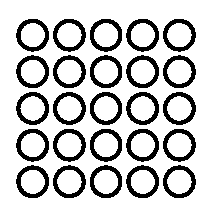
\includegraphics{figure/fig40.eps}
\end{figure}

sama caturada rAshiya guMDugaLanunx kANuva mAgaR.

I rAshiyanunx ideV riVtiyAgi peVrisutAtx hoVguvAgeyx nAlukx nAlukx
guMDugaLa meVle oMdoMdu guMDugaLa parxkArakekx sAthxpitavAgi,
meVlagaDe oMdu guMDu yAvAgeyx nilulxtatxdeyoV Ageyx I rAshi
samanAyiteMdu tiLiya beVku.

\begin{verse}
sUtarx|| aDi sAlina guMDugaLoLu| taDeyade sheVrisuta loMda noMduM
sheVrida|| aDi sAlinxMmaDiyoVLiri| daDisAliMdiridu labadhx
mAraroLahxriseY|| 

vi|| taLadalilx oMdu pAshavxRdalilx sAlagiruva guMDugaLa saMKayxdalilx
$1$ sheVrisi adanunx adeV sAlina guMDugaLa divxguNadalilx $1$
sheVridadxriMda guNisi A labadhx vanunx punaH adeV sAlina guMDugaLa
saMKayxdiMda guNisi baMda labadhxvanunx $6$riMda BAgisidare, guMDugaLa
oTuTx parxmANagaLAguvadu.

riVti, meVlina rAshiya taLada sAlinalilx pAshavxR oMdakekx $5$
guMDugaLiruva kAraNa,
$$
\frac{(5+1)(10+1)\times 5}{6}=55\text{~ guMDugaLu utatxra.}
$$ 

sUcane|| $1$, $4$, $9$, $16$, $25$ I vidhavAda vagoRVtatxra vaqdidhxya
saravxdhanavanunx kANuva mAgaRvAgirutatxde.
\end{verse}

\medskip
\begin{center}
{\large\bf 162neV aBayx udAharaNe.}
\end{center}

\begin{itemize}
\item[\rm(1)] oMdu cacwkavAda guMDina rAshiya taLada sAloMdakekx $50$
guMDugaLidadxre, A rAshiyalilx oTuTx guMDugaLeSiTxra bahudu?

\item[\rm(2)] $1$, $4$, $9$, $14$ itAyxdi vagoRVtara vaqdidhxyalilx
$30$ gaCa padagaLidadxre, saravx dhana eSATxguvadu?
\end{itemize}



\chapter{146neV parxkaraNa}

\begin{center}
{\large\bf tirxkoVNa kaqtiya rAshigaLa guMDugaLanunx kANuva mAgaRvu.}
\end{center}

\begin{figure}[H]
\centering
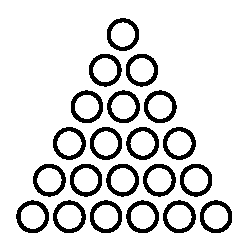
\includegraphics{figure/fig41.eps}
\end{figure}

I rAshiyanunx ideV riVtiyAgi peVrisutAtx hoVdare, mUru mUru guMDugaLa
meVle oMdoMdu guMDugaLa parxkArakekx sAthxpitavAgi meVlagaDe oMdu
guMDu niMtu koMDare, I vidhavAda rAshiyu saMpUNaRvAyiteMtA tiLiya
beVku.

\begin{verse}
sUtarx|| taLaleKa doLoMda sheVrisi| taLadoLu matetxraDa sheVri
sutatxdaniridu|| taLaleVKada Liriyutatxda| tiLidAra roLahxrisa labadhx
goVLa parxmANaM||

vi|| taLada sAlina guMDina leKaKxdalilx $1$ sheVrisi adanunx $2$
sheVrisidaMthA taLa sAlina saMKayxdiMda guNisi punaH adanunx taLa
sAlina guMDugaLa saMKayxdiMda guNisi labadhxvanunx $6$riMda BAgisu.
$$
\frac{(6+1)(6+2)\times 6}{6}=56\text{~ guMDugaLa parxmANavu.}
$$

sUcane|| idu $1$, $3$, $6$, $10$, $15$, $21$ I riVtiyAda sherxVNigaLa
saravx dhanavanunx kANuva mAgaRvAgirutatxde.
\end{verse}

\medskip
\begin{center}
{\large\bf 163neV aBayx udAharaNe.}
\end{center}

\begin{itemize}
\item[\rm(1)] oMdu tirxkoVNA kaqtiyuLaLx guMDina rAshiya taLaBAgada
oMdu pAshavxRdalilx $100$ guMDugaLidadxre, A rAshiyalilx oTuTx
guMDugaLeSiTxra bahudu?

\item[\rm(2)] $1$, $3$, $6$, $4$, $15$ I riVtiyAda sherxVNiya gaCaCx
padagaLu $75$ idadxre, saravx dhana eSATxguvadu?
\end{itemize}


\chapter{147neV parxkaraNa}

\begin{center}
{\large\bf AyakeSxVtArx kaqtiyAgi peVrisidaMthA guMDina rAshiya guMDugaLa}
\vskip .3cm

{\large\bf parxmANavanunx kANuva mAgaRvu.}
\end{center}

\begin{figure}[H]
\centering
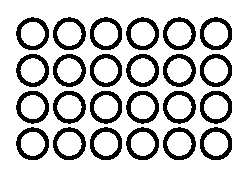
\includegraphics{figure/fig42.eps}
\end{figure}

idanunx peVrisuvAgeyx nAlukx nAlukx guMDugaLa meVle oMdoMdu guMDugaLa
parxkArakekx nilulxtAtx meVlagxDeV sAlage oMdoMdeV guMDugaLu
niMtukoLuLxvavu. 

\medskip
\begin{center}
{\large\bf sUtarx.}
\end{center}

\begin{verse}
kaM|| udadxdataLa tirxguNadoLuM| badidhxsutoMdadaroLagala
sAlinaleKaM|| badadhxdi kaLaduLidudanA| gidadxgaladoLoMdakUDi
shidadxroLiridU|| 

badadhxdi baMdA labadhxva| nidadxgalado LiriyutAga baMdArAshiya||
shudadhxdoLAraroLahxrisalf| nidadhxRradiM bakukxvasana rAshiyaguMDU||

vi|| udadxvAda taLada sAlina guMDugaLa saMKayxda tirxguNadalilx $1$
sheVrisi, adaralilx agalada taLa sAlina guMDugaLa saMKayxvanunx
kaLadu, uLidadadxnunx A yagalada taLa sAlina guMDugaLa saMKayxdalilx
$1$ sheVrisidadxriMda guNisi, adanunx punaH agala sAlina taLada
leKaKxdiMda guNisi, labadxvanunx $6$riMda BAgisu.
$$
\frac{(18+1-4)(4+1)\times 4}{6}=50\text{~ guMDugaLU.}
$$
\end{verse}

\medskip
\begin{center}
{\large\bf 164neV aBayx udAharaNe.}
\end{center}

\begin{itemize}
\item[\rm(1)] oMdu Aya keSxVtArx kaqtiyAda guMDina rAshiya udadxda
taLada parxmANadalilx $50$ guMDugaLU matutx agalada kaDeV $30$
guMDugaLu uLaLxdAdxgidadxre, A rAshiya oTuTx guMDugaLeSiTxra bahudu? 
\end{itemize}


\chapter{148neV parxkaraNa}

\begin{center}
{\large\bf davasada rAshigaLalilx iSuTx parxmANa davasagaLirutatxve}
\vskip .3cm

{\large\bf eMdu kaMDu hiDiyuva mAgaRvu.}
\end{center}

\begin{verse}
kaM|| pirikALige dashamAMshaM| kiridakekxVkAdashAMshasuMkAkxdudakaM||
diruvadu navamAMshavukeV| Lapxri\-dhiya niVLaMga LaLate parimitigaNaka||

vi|| pirikALeMdare, avare, haraLu, ududx, togari, modalAda
dhAnayxgaLidadxre, A rAshigaLa paridhiya $\frac{1}{10}$ BAgavu
niVLavirutatxdeMtalU, kiri kALeMdare, rAgi, sAsuve, huraLi modalAda
dhAnayxgaLAgidadxre, A rAshiya paridhiya $\dfrac{1}{11}$ BAga niVLa
virutatxdeMtalU, suMkakx dhAnayxveMdare, goVdhi, Batatx, navaNe,
itAyxdi dhAnayxgaLa rAshiyAdare, adara paridhiya $\frac{1}{9}$ BAga
niVLa virutatxdeMtalU tiLiya beVku. niVLaveMdare, A rAshigaLa madhayx
parxmANada unanxtavu.
\end{verse}

\begin{center}
{\large\bf sUtarx.}
\end{center}

\begin{verse}
kaM|| rAshiya paridhiya naLadA| rAshiya dhAnayxgaLa bageya
nariyutaniLadiM|| rAshiya paridhiya \hbox{SaDABx|} gAsuradiM dogaRgoMDa
saMKayxva niridU||

rAshiya paridhiya moLakaM| rAshiyo LeMBatutx sheVru iruva parxmANaM||
leVsiMdari yutatxdakaM| dAsamayadi rAshi karxyada gaNitadi noVDeY||

vi|| eMthA rAshigaLAdAgUyx adara paridhigaLanunx dhAradiMda aLateV
mADi, A rAshige takakx niVLagaLanunx meVle heVLiruva parxkArakekx
sAdhisikoMDu A niVLa saMKayxgaLanunx A rAshiya paridhiya $\frac{1}{6}$
BAgada vagaRdiMda guNasidare, aSuTx Gana aMgulagaLAguvavu. taruvAya,
$24$ Gana aMgulagaLige $80$ sheVrugaLAdare, A baMdaMthA Gana
aMgulagaLige eSATxdiVteMdu terxY rAshiyiMda noVDikoMDu baMdaMthA Pala
sheVrugaLige KaMDi athavA palAlx, modalAdavugaLanunx mADa bahudu.
\end{verse}

\begin{figure}[H]
\centering
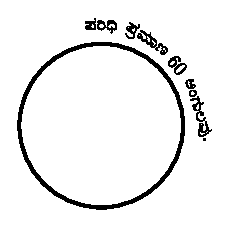
\includegraphics{figure/fig43.eps}
\end{figure}

Agalu, paridhi $60\times \frac{1}{10}=6$ aMgula dapapx kALina niVLavu.

paridhi $60\times \frac{1}{11}=5\frac{5}{11}$ aMgula saMNa kALina
niVLavu.

paridhi $60\times \frac{1}{9}=6\frac{2}{3}$ suMkAda dhAnayxda niVLavu.

dapapx kALige|| Agalu, paridhi $60$ idara $\frac{1}{6}$ BAga $10$
idara vagaRvu $100\times 6$ niVLa $=600$ Gana aMgula.

saMNa kALige|| matutx paridhi $60$ idara $\frac{1}{6}$ BAga $10$
vagaRvu $100\times \frac{60}{11}=\frac{6000}{11}=545\frac{5}{11}$ Gana
aMgula. 

suMkikxge|| paridhi $60$ idara $\frac{1}{6}$ BAga $10$ vagaRvu
$100\times \frac{20}{3}=\frac{2000}{3}=666\frac{2}{3}$ Gana aMgula.

Agalu terxYrAshiyu.
\begin{center}
\begin{tabular}{c@{\,:\,}c@{\,::\,}cl}
aMgulakekx & sheVru & ke. & \\[3pt]
$24$ & $80$ & $600$ & $=2000$ sheVru dapapx kALugaLa parx.\\[3pt]
$\frac{24}{1}$ & $\frac{80}{1}$ & $\frac{6000}{11}$ &
$=1818\frac{2}{11}$ sheVru saMNakALugaLa parx.\\[3pt]
$\frac{24}{1}$ & $\frac{80}{1}$ & $\frac{2000}{3}$ &
$=2222\frac{2}{9}$ sheVru suMku dhAnayx parx.
\end{tabular}
\end{center}

\begin{verse}
sUcane|| mUleyalilx surida rAshiyu saMpUNaR rAshiya, $\frac{1}{4}$
BAgaveMtalU goVDeV pAshavxRkekx surida rAshiya saMpUNaR rAshiya
$\frac{1}{2}$ BAga veMtalU tiLiya beVku. 
\end{verse}

\medskip

\begin{center}
{\large\bf 165neV aBayx udAharaNe.}
\end{center}

\begin{itemize}
\item[(1)] $54$, $72$, $96$ aMgula parxmANa paridhigaLuLaLx avare,
matutx rAgi, hAgU Batatx I vidhavAda mUru dhAnayxgaLa rAshigaLanunx
suradidadxre, A rAshigaLalilx yAvAyxva dhAnayxgaLu eSeTxSiTxra bahudu,
heVLu? 
\end{itemize}


\chapter{149neV parxkaraNa}

\begin{center}
{\large\bf gaqhAMka sAthxpanA karxmavu.}
\vskip .3cm

{\large\bf viSamavAda gaqhagaLige aMkasAthxpanA karxmavu.}
\end{center}

aMdare, mUrAdiyAda viSama gaqhagaLige $1$ra modalogxMDu
varaseyAgiyAgali, vaqdidhx karxmavAgi yAgaliV aMkegaLanunx baradu
avugaLa sAlugaLanunx kUDisidare, oMdeV samanAda oTuTx leKaKxgaLu
baruvaMthA mAgaRvu.

\medskip
\begin{center}
{\large\bf sUtarx.}
\end{center}

\begin{verse}
kaM|| meVlina madhayxdoLoMdaM| kiVLinoLeraDadara
yeDadamuMduMkarxmado|| LUmxleya naDarutanaMtara| sAlina kaDe
madhayxdiMda mUleyanaDareY||

taDadare kiVLimAmxyXla| kokxDanoDaneV sAthxpisutatx mUlegepoVgu||
totxDane bala BAga meVlipxno| LadxDigaDigaM sAthxpisutatx kUDalu
samaneY|| 

vi| modalu meVlagxDeV sAlina madhayxdalilx $1$nunx adara eDagaDeV
sAlina keLagaDeV maneyalilx $2$nUnx alilxMdA mUlegaLanunx aDarutAtx
karxmAMkigaLanunx baradu, A meVle balagaDeV sAlina madhayxda
modalogxMDu mUlegaLananxDari bariyutAtx taDadare, adara keLagaDeV
maneyiMda punaH bala\-gaDeV meVlABxgada mUlegaLanunx aDari bariyutAtx
punaH punaH adeV karxmavAgi sAthxpisutAtx manegaLanenxlAlx mugisa
beVku. 
\end{verse}

\begin{center}
\renewcommand{\arraystretch}{1.2}
\begin{tabular}{|>{\rm}r|>{\rm}r|>{\rm}r|}
\hline
6 & 1 & 8\\
\hline
7 & 5 & 3\\
\hline
2 & 9 & 4\\
\hline
\end{tabular}
\end{center}

riVti| ililx meVlina sAlina madhayxdalilx $1$ nunx adara eDagaDeV
sAlina keLagina maneyalilx $2$nUnx baradu, muMde balaBAgada madhayxda
maneyalilx $3$nunx baradu, taDadadxriMda adara keLage $4$ baradu,
mUleyanunx aDarutAtx $5$, $6$, $7$nunx baradu, A meVle balaBAgada
meVlina maneyalilx $8$nunx baradu punaH keLakikxLidu $9$nunx
baradirutatxde. 

\begin{center}
\renewcommand{\arraystretch}{1.2}
\begin{tabular}{|>{\rm}r|>{\rm}r|>{\rm}r|>{\rm}r|>{\rm}r|>{\rm}r|}
\hline
15 & 8 & 1 & 24 & 17\\
\hline
16 & 14 & 7 & 5 & 23\\
\hline
22 & 20 & 13 & 6 & 4\\
\hline
3 & 21 & 19 & 12 & 10\\
\hline
9 & 2 & 25 & 18 & 11\\
\hline
\end{tabular}
\end{center}

ililx meVlina madhayxda maneyalilx $1$ baradu, alilxMdA adara
yaDagaDeV sAlina keLagaDeV maneyalilx $2$ nunx baradu, meVlina
mUleyalilx $3$nunx baradu, alilxMdA bala BAgada madhayxdalilx $4$nunx
sAthxpisi, adara meVlina mUleyalilx $5$ bariyalAgi taDeyAdadxriMda
adara keLage $6$nunx baradu, mUlegaLa varaseV meVrige $7$, $8$nunx
baradirutatxde. alilxMdA punaH eDa BAgada keLagina maneyalilx $9$nunx
baradu punaH balakekx tirugi $10$nunx baradu, taDadadxriMda adara
keLage $11$nunx muMde mUlegaLa varaseV parxkArakekx $12$, $13$, $14$,
$15$, $16$nunx baradu, biTuTx, alilxMdA bala BAgada meVlina maneyalilx
$17$nunx baradu punaH adara eDa BAgada keLagina maneyalilx $18$nunx
muMde mUlegaLalilx $19$, $20$nunx baradu taDadadxriMda, adara keLage
$21$nunx mUleyalilx $22$nunx baradu, punaH bala BAgakekx tirigi $23$,
$24$nunx baradu, adara eDagaDeV sAlina keLagina maneyalilx $25$nunx
baradirutatxde. 

\begin{verse}
sUcane|| I manegaLige aMkikxgaLanunx bariyuvAgeyx sUtarx karxmavanunx
jAcnxpakadalilxTuTxkoMDu nAlAkxvatiR maMdaTuTx mADikoMDare, A meVle
eSuTx manegaLige beVkAdAgUyx sarAgavAgi bariya bahudu. ideV
karxmadalilx vaqdidhxgaLAgi aMkegaLanunx baradAgUyx sari baruvadu. 
\end{verse}

\medskip
\begin{center}
{\large\bf 166neV aBayx udAharaNe.}
\end{center}

\begin{itemize}
\item[\rm(1)] obabx reYtanalilx oMdAdiyAgi EkoVtatxra vaqdidhxyAgi
$9$ra varigU kaTiTxdaMthA $9$ mUTe kALugaLidadxvu. avugaLanunx avanu
tananx mUru jana makakxLige dhAnayxgaLu sariyAgi baruva hAgU, mUTegaLu
samanAgiruva hAgU haMci koDa takakxdudx hAyxge?

\item[\rm(2)] obabxnu oMdAdiyAgi EkoVtatxra vaqdidhxya karxmavAgi
hAlanunx kariya takakxMthA $25$ hasugaLanunx tananx $5$ jana
makakxLugaLige hAlugaLu sariyAgi baruva hAge aideYdu hasugaLanunx
haMci koDa beVkAda vidha hAyxge?
\end{itemize}

\medskip
\begin{center}
{\large\bf parxkAra $2$.}
\end{center}

\begin{center}
{\large\bf viSama gaqhagaLalilx koVridaSuTx labadhx baruva hAge aMkigaLanunx}\\
\vskip .2cm
{\large\bf vaqdidhx karxmavAgi bariya beVkAdare, modalu eraDaneV mane}\\
\vskip .2cm
{\large\bf ge bariya takakx labadhxvanunx kANuva mAgaRvu.}
\end{center}

\begin{verse}
sU|| irutiha manegaLa leKava| nirisAli noLadhaRdiMdalA sAladhaRva||
koratisu tutatxraviridada| naritiCeCxyo LaLidusAla
saMKayxdoLahxriseY||

vi|| manegaLa leKaKxvanunx adara sAlina adhaRdiMda guNisi,
labadhxdalilx A manegaLa sAlina adhaRvanunx kaLadu, sheVSavanunx
utatxra saMKayxdiMda guNisi labadhxvanunx iCeCxya labadhxdalilx kaLadu
uLidadadxnunx sAlina saMKeyxyiMda BAgisu, baruva labadhxveV modalaneV
manege bariyuva saMKayxvAgiruvadu. adanunx $2$neV manege baradu, muMde
vaqdidhxsutAtx meVlina sUtarxkarxmavAgi yalAlx manegaLigU baradare
sariyAguvadu. 
\end{verse}

riVti,

\begin{minipage}[c]{5cm}
\begin{center}
\renewcommand{\arraystretch}{1.2}
\begin{tabular}{c|r|r|r|}
\cline{2-4}
& $30$ & $5$ & $40$\\
\cline{2-4}
& $35$ & $25$ & $15$\\
\cline{2-4}
& $10$ & $45$ & $20$\\
\cline{2-4}
\multicolumn{1}{c}{oTuTx} & \multicolumn{1}{r}{$75$} & \multicolumn{1}{r}{$75$}
& \multicolumn{1}{r}{$75$} 
\end{tabular}
\end{center}
\end{minipage}
\qquad
\begin{minipage}[c]{5cm}
\begin{center}
\renewcommand{\arraystretch}{1.2}
\begin{tabular}{c|>{\rm}r|>{\rm}r|>{\rm}r|>{\rm}r|>{\rm}r|}
\cline{2-6}
 & 68 & 40 & 12 & 104 & 76\\
\cline{2-6}
 & 72 & 64 & 36 & 28 & 100\\
\cline{2-6}
 & 96 & 88 & 60 & 82 & 24\\
\cline{2-6}
& 20 & 92 & 84 & 56 & 48\\
\cline{2-6}
& 44 & 16 & 108 & 80 & 52\\ 
\cline{2-6}
\multicolumn{1}{c}{oTuTx} & \multicolumn{1}{r}{$300$}
& \multicolumn{1}{r}{$300$} & \multicolumn{1}{r}{$300$}
& \multicolumn{1}{r}{$300$} & \multicolumn{1}{r}{$300$} 
\end{tabular}
\end{center}
\end{minipage}

\begin{itemize}
\item[\rm(1)] udAharaNe, mUru manegaLa labadhxvu $75$ baruvaMteyU
oMdakikxMtA matotxMdu maneya aMkigaLu aideYdu hecAcxgiruvaMteyU A $9$
manegaLigU aMkigaLanunx bari?

\item[\rm(2)] aideYdu manegaLa oTuTx labadhxvu $300$ baruvaMteyU
oMdakikxMtA matotxMdu maneya aMki nAlukx nAlukx hecAcxgiruvaMteyU A
$25$ manegaLigU aMkigaLanunx bari?
\end{itemize}

\begin{tabular}{lc@{\qquad}c}
\multicolumn{2}{c}{riVti, ($1$neVdu) manegaLu $9$ sAlu $3$} &
($2$neVdu) manegaLu $25$ sAlu $5$\\[4pt]
\qquad guNisalu & $27$ & $125$\\[2pt]
\qquad adhiRsalu & $13\frac{1}{2}$ & $62\frac{1}{2}$\\[2pt]
\qquad maneya salina adhaRgaLu & $1\frac{1}{2}$ & $2\frac{1}{2}$\\[2pt]
\qquad kaLiyalu & $12$ & $60$\\[2pt]
\multicolumn{2}{l}{\qquad avugaLanunx vaqdidhx eMba utatxradiMda guNisalu}\\[2pt]
 & $5$ & $4$\\[2pt]
\qquad labadhxvu & $60$ & $240$\\[3pt]
\multicolumn{2}{p{5.5cm}}{iCACx labadhx $75-60=15\div$ sAlu $3=5$ idu
modalu manege bariya takakxdu.} &
\multicolumn{1}{p{6cm}}{iCACx labadhx $300-240=60$\quad $60\div 5$
sAlu $=12$ idu modalu bariya takakxdu.}
\end{tabular}

\medskip
\begin{center}
{\large\bf 167neV aBayx udAharaNe.}
\end{center}

\begin{itemize}
\item[\rm(1)] obabx dhoreyu tananx $9$ jana makakxLige tanige
sheVridaMthA $25$ varahA modalogxMDu aideYdu varahAgaLu hecucx
hecAcxgi huTuTxvaLiyuLaLxMthA $81$ gArxmagaLanunx huTuTxvaLi elalxrigU
samanAgi baruva hAge obobxbabxnige $9$ gArxmagaLu baruva hAge haMci
koDa takakxdudx hAyxge?
\end{itemize}


\chapter{149neV parxkaraNa}

\begin{center}
{\large\bf SoVDasha gaqhAMka sAthxpane.}
\end{center}

aMdare, $4$ sAlugaLuLaLx $16$ manegaLige sAloMdakekx iSuTx oTuTx bara
beVkeMba nibaMdhanege sariyAgi aMkegaLanunx bariyuva karxmavu.

\medskip
\begin{center}
{\large\bf parxkAra $1$}

\bigskip

{\large\bf sUtarx.}
\end{center}

\begin{verse}
kaM|| iSaTxva nadhiRsutoMdoM| daSaTxroLuM kaLaducaraNa
navaSoVDashasa|| patxSATxdipUNiRmadashameV| kiSaTxku bariyutatxluLiva
gaqhadoVLakxrXmadiM|| 

karasapatx SaTakxrAmaM| duritaM soVmAbidhx bANa nirutaM sAthxpisu|
taritaritu catura gaqhagaLa| tarataradiM kUDisalekx samanaMtakukxM||

vi|| $4$ manegaLanunx kUDidare, eSuTx labadhxvAga beVkoV adanunx
adhiRsi, adaralilx oMdoMdanunx kaLiyutAtx $2$, $9$, $16$, $7$, $8$,
$15$, $10$, $1$ I manegaLige baradu uLida manegaLige karxmavAgi $2$,
$7$, $6$, $3$, $8$, $1$, $4$, $5$ aMkegaLanunx baradare samanAguvadu. 
\end{verse}

\begin{center}
\renewcommand{\arraystretch}{1.2}
\begin{tabular}{|>{\rm}r|>{\rm}r|>{\rm}r|>{\rm}r|}
\hline
17 & 24 & 2 & 7\\
\hline
6 & 3 & 21 & 20\\
\hline
23 & 18 & 8 & 1\\
\hline
4 & 5 & 19 & 22\\
\hline
\end{tabular}
\end{center}

u. sAloMdakekx $50$ oTuTx baruva hAge ililx kANisiruva $16$ manegaLigU
aMkegaLanunx bari? riVti, $50$ adhaRvu $25-1=24$ eraDaneV manegu,
muMde $23$, $22$, $21$, $20$, $19$, $18$, $17$nunx $2$, $9$, $16$,
$7$, $8$, $15$, $10$, $1$neV manegaLigU baradu ide. A meVle $2$, $7$,
$6$, $3$, $8$, $1$, $4$, $5$ ivugaLanunx karxmavAgi baradide. 

\newpage

\begin{center}
{\large\bf 168neV aBayx udAharaNe.}
\end{center}

\begin{itemize}
\item[\rm(1)] oMdakiMtAtx oMdu oMdoMdu varahAtUka kaDameyAgi
mADisidaMthA $8$ uMgaragaLu obabxnalilxdadxvu. Aga avanu punaH
$1$kiMtAtx oMdu oMdoMdu varahA tUka hecAcxdaMthA $8$ uMgaragaLanunx
mADisi, obobabxrige $120$ varahA tUkagaLu sariyAgi baruva hAge tananx
$4$ jana makakxLige haMcikoTaTxnu. Agalu, A uMgarxgaLa
tUkagaLeSeTxSuTx? matutx avanu haMci koTaTx vidha hAyxge?
\end{itemize}

\medskip
\begin{center}
{\large\bf parxkAra $2$}\\
\vskip .2cm
{\large\bf eSATxdarU vaqdidhxya karxmavAgi $16$ manegaLige aMkegaLanunx}\\
\vskip .2cm
{\large\bf baradare, $4$ manegaLa oTuTx oMdeV samanAgi}\\
\vskip .2cm
{\large\bf bara takakxMthA mAgaRvu.}
\end{center}

\begin{verse}
sUtarx|| karanavaSoVDashasapatxM|
karipakaSxMdashamicaMderxVkAdashacatura|| shashxrama nutirx
dashASaTaTxM| pura\-ravi gaqhasAthxpisalekx samanaMtakukxM||

vi|| $1$ AdiyAgi, $2$, $9$, $16$, $7$, $8$, $15$, $10$, $1$, $11$,
$4$, $5$, $14$, $13$, $6$, $3$, $12$ I manegaLige EkoVtatxra
vaqdidhxyAgi baradare, sariyAguvadu.
\end{verse}

\begin{center}
\renewcommand{\arraystretch}{1.2}
\begin{tabular}{r|>{\rm}r|>{\rm}r|>{\rm}r|>{\rm}r|}
\cline{2-5}
 & 8 & 1 & 15 & 10\\
\cline{2-5}
 & 11 & 14 & 4 & 5\\
\cline{2-5}
 & 2 & 7 & 9 & 16\\
\cline{2-5}
 & 13 & 12 & 6 & 3\\
\cline{2-5}
\multicolumn{1}{c}{oTuTx} & \multicolumn{1}{r}{$34$}
& \multicolumn{1}{r}{$34$} & \multicolumn{1}{r}{$34$}
& \multicolumn{1}{r}{$34$} 
\end{tabular}
\end{center}


u. $1$ AdiyAda EkoVtarx vaqdidhxya karxmavAgi belegaLuLaLx $16$
vasatxrXgaLanunx $4$ janagaLige sariyAgi belegaLu baruva hAge
vasatxrXgaLanenxV haMcikoDuva vidha hAyxge?

matutx obobxbabxnige eSuTx beleyuLaLx vasatxrXgaLu baMdAvu?

\medskip
\begin{center}
{\large\bf iCAcx labadhx bara takakxdadxkekx sUtarx.}
\end{center}

\begin{verse}
kaM|| modaliMdavxqqdidhxge sAthxpisi| tadanaMtara
sAlakUDaleSATxguvadada| mudadiCeCxya leKadoLaLi| dadanAlekxroLahxrisu
toMda kUDutaladanaM||

muMdinayusamx gaqhadoV| LacxMdadi bariyutatx niMda gaqhagaLigelalx|
kakxMdadi vaqdidhxsi bariyuta| laMdava kUDalekx yiSaTx
sariyAgikukxRM||

udAharaNeyu, obabx dhoreyu sAloMdakekx $4$ lAyagaLuLaLx $16$
lAyagaLalilxyU tananx kuduregaLanunx, oMdakiMtAtx matotxMdaralilx
aideYdu kuduregaLu hecAcxgiruvaMteV kaTiTxsi, A meVle oMdoMdu sAlina
$4$, $4$ lAyagaLanenxV tananx makakxLige koTuTxbiTaTxnu. Aga
obobxbabxrige $1270$ kuduregaLa parxkArakekx shikikxdavu. Agalu,
eSeTxSuTx kuduregaLanunx kaTiTxdaMthA lAyagaLu yArAyxrigeSeTxSuTx
baMdavu, heVLu?

vi|| ililx $5$ra vaqdidhxya meVrige kaTaTxlAgi sAloMdakekx $1270$
idadxveMba athaRvAyitu. AdadxriMda modalu $5$ra vaqdidhxya karxmavAgi
muMcina sUtarxda parxkArakekx aMkegaLanunx sAthxpisi sAloMdakekx
eSATxdiVteMbuvadanunx tiLadukoMDu, adanunx iCACx labadhxdalilx kaLadu
uLidadadxnunx $4$riMda \hbox{BAgisi} labadhxdalilx $1$ kUDisidare, adu $2$neV
manege bariyuva leKaKxvAgiruvadu. anaMtara, \hbox{vaqdidhxya} parxkArakekx
hecicxsutAtx modalina sUtarxdaMteyeV, $2$, $9$, $16$, $7$, $8$, $15$,
$10$, $1$, $11$, $4$, $5$, $14$, $13$, $6$, $3$, $12$ manegaLalilx
bariyutAtx hoVdare, iCACx labadhxkekx sari baruvadu. 
\end{verse}

\begin{center}
\renewcommand{\arraystretch}{1.2}
\begin{tabular}{|>{\rm}r|>{\rm}r|>{\rm}r|>{\rm}r|}
\hline
36 & 1 & 71 & 46\\
\hline
51 & 66 & 16 & 21\\
\hline
6 & 31 & 41 & 76\\
\hline
61 & 56 & 26 & 11\\
\hline
\end{tabular}
\end{center}

I riVtiyAgi sAthxpisalu, sAloMdakekx $154$ barutatxde. Agalu, namige
baratakakx iCACxlabadhxvu $1270$ AdadxriMda, $1270-154=1116$ idanunx
$4$riMda BAgisalu $279$ idaralilx $1$ sheVrisalu $280$ idu eraDaneV
manege bariya beVkAda labadhxvu.\qquad Agalu,

iCACx labadhxkekx
\begin{center}
\renewcommand{\arraystretch}{1.2}
\begin{tabular}{|>{\rm}r|>{\rm}r|>{\rm}r|>{\rm}r|}
\hline
315 & 280 & 350 & 325\\
\hline
330 & 345 & 295 & 300\\
\hline
285 & 310 & 320 & 355\\
\hline
340 & 335 & 305 & 290\\
\hline
\end{tabular}
\end{center}

ililx $2$neV maneyalilx $280$nunx baradu muMde sUtarx parxkArakekx
$9$, $16$, $7$, $8$, $15$, $10$, $1$, $11$, $4$, $5$, $14$, $13$, $6$,
$3$, $12$neV manegaLalilx aideYdanunx hecicxsi baradirutatxde. Aga,
kUDisalu iCACx labadhx $1270$ Aguvadu.

\medskip
\begin{center}
{\large\bf 169neV aBayx udAharaNe.}
\end{center}

\begin{itemize}
\item[\rm(1)] obabx ja\!\,{ha}girfdAranu paMcoVtatxra vaqdidhxyAgi
huTuTxvaLigaLiratakakxMthA $16$ gArxmagaLanunx tananx $4$ jana
makakxLige gArxmagaLu sariyAgi bruvaMteyU huTuTxvaLi obobxbabxrige
$2000$ rUpAyigaLu sariyAgiruvaMteyU haMci koTaTxnu. Aga A gArxmagaLa
huTuTxvaLi eSeTxSuTx? matutx haMci koTaTx vidha hAyxge?
\end{itemize}


\chapter{150neV parxkaraNa}

\begin{center}
{\large\bf sUtarx gaNitagaLanunx kuritadudx.}
\end{center}

kelavu vinoVdavAgiyU, AshacxrayxvAgiyU ita takakx leKaKxgaLige
parxteyxVkavAda sUtarxgaLanunx kalipxsi sulaBavAgi aMthA jAtiV
leKaKxgaLanenxlAlx mADavadakokxVsakxravAgi I keLage bariyalapxDuvavu.



\chapter{151neV parxkaraNa}

\begin{center}
{\large\bf nUyxnAdhika samIkaraNada leKaKxvu.}
\end{center}

\begin{verse}
{\rm(1)}~ u. parxti divasavU $8$ gAvadavanunx naDiya takakxvanu horaTa
$12$ divasada meVle parxti divasavU $32$ gAvadavanunx naDiyatakakxvanu
horaTare, avaribabxrU eSuTx divasagaLalilx saMdhishAyxru, heVLu?

sUtarx|| modalina gAvadadivasava| mudadiMdiriyutatx baMda
labadhxvanAgalf|| modaleraDane gAvadagaLi| godagutihAMtatxradoLahxrisu
baMdude divasaM||

vi|| modalaneVyavanu naDiya takakx gAvadagaLanunx eraDaneVyavanu
horaTa divasadiMda guNisi, A labadhxvanunx A uBayatarxra gamanAMtara
saMKeyiMda BAgisidare, saMdhisida divasagaLAguvavu.
\end{verse}

\hfill modalenxyavana gamana $8$ gAvada $\times 12$ eraDaneVyavanu horaTa
divasa $=96$

\hfill $32-8=24$ idu gamanAMtaravu. Agalu $\frac{96}{24}=4$

\hfill divasakekx saMdhisidaru.


\chapter{152neV parxkaraNa}

\begin{center}
{\large\bf puSapxda leKAKx.}
\end{center}

\begin{verse}
{\rm(1)}~ u. mUru deVvasAthxnagaLU matutx $3$ saroVvaragaLu
idadxvu. obabx pUjAriyu kelavu puSapxgaLanunx taMdu $1$neV
saroVvaradalilx adadxlAgi $1$kekx nAlakxraSuTx hecicxdavu, avugaLalilx
kelavu puSapxgaLanunx $1$neV guDiyalilx aciRsi uLidadadxnunx $2$neV
saroVvaradoLage adudxvAgeyx $1$kekx $7$raSuTx hecicxdavu. Aga
avugaLalilx modala guDiyalilx eSuTx puSapxgaLanunx acicxRsidadxnoV
aSeTxV puSapxgaLanunx pUjisi, uLidadadxnunx $3$neV saroVvaradalilx
adadxlAgi $1$kekx $9$raSuTx hecAcxdavu, avugaLanunx $3$neV
deVvasAthxnadalilx muninxnaMteyeV samapiRsalAgi sheVSa
uLiyalilalxvU. Adare, avanu Adiyalilx taMda puSapxveSuTx? matutx
oMdoMdu guDigaLalilx pUjisida puSapxgaLa saMKeyx yeSuTx, heVLu? 

sUtarx|| eMtiha maDigaLeniriya| labxMtenisida labadhxguDi gapiRsutiha
puSapxM|| aMtumodaloMdabiTATx| geMtihamaDiguDiyagUDimaDiyiMguNiseY|| 

vi|| vaqdidhxyAda saMKayxgaLa guNAkAravu oMdoMdu guDigapiRsida
puSapxveMtalU A maDigaLa saMKayxdalilx modalaneV maDiyanunx biTuTx
uLida maDi saMKayxdalilx guDiyanunx kUDisi, punaH maDi saMKayxdiMda
guNisi, adaralilx guDi saMKayxvanunx kUDisutAtx hoVdare, Adiya puSapx
doriyuvadeMtalU tiLiya beVku. 
\end{verse}

\begin{center}
\begin{tabular}{l@{\qquad\qquad}c|cc@{\qquad}l}
riVti, & $1$ & $1$ & $1$ & guDigaLu\\[3pt]
Agalu & $4$ & $7$ & $9$ & maDigaLu
\end{tabular}
\end{center}

Agalu
$$
4\times 7\times 9=252\quad\text{idu oMdoMdu guDiyalilx apiRsida puSapxvu.}
$$

$7+1$ guDi $=8\times 9$ maDi $=72+1$ guDi $=73$ idu Adiyalilx taMda
puSapxvu. 

hiVge eSuTx guDigaLu, eSuTx maDigaLigAdAgUyx mADa bahudu.


\chapter{153neV parxkaraNa}

\begin{center}
{\large\bf dAriyalilx kaMDa darxvayxda gaMTina leKAKx.}
\end{center}

\begin{verse}
{\rm(1)}~ u. aMNa, tamamxMdiru dAriyanunx naDiyutitxralAgi oMdu
darxvayxda gaMTanunx kaMDaru. adanunx bicicx, A darxvayxvanUnx aMNanu
tegadukoMDu tananxlilxdadx darxvayxvanUnx sheVrisi tamamxna keYlidadx
darxvayxkekx mUraraSATxguteMdu heVLidanu. Aga tamamxnu adeV gaMTina
darxvayxvanunx tAnu tegadukoMDu tananxlilxdadx darxvayxvanunx sheVrisi
aMNanalilxdadx darxvayxda imamxDi yAgutetxMdu heVLidanu. Adare, Aga
avarugaLalilxdadx darxvayxgaLeSuTx matutx shikikxda gaMTinalilxdadx
darxvayxgaLeSuTx? 

sUtarx|| maDigaLa niriyutaloMdanu| taDeyilalxdekaLiyalAga
gaMTinadarxvayxM|| mADigaLoLagoMda kUDisa| loDanadu dArigaroLidadx
davayxparxmANaM||

vi|| avarugaLu toVrisada maDigaLa saMKegaLanunx guNisi A labadhxdalilx
$1$ kaLadare gaMTinalilxdadx darxvayxvU, matutx A maDigaLa
saMKayxgaLalilx parxteyxVka parxteyxVkavAgi $1$nunx sheVrisidare,
avaravara, keYlidadx darxvayx parxmANagaLU baruvavu.
\end{verse}

\begin{align*}
& 3\text{~ maDi~ }\times 2\text{~ maDi~}=6-1=5\text{~ idu shikikxda
darxvayx parx.}\\[5pt]
& \frac{1}{4}\text{~ aMNanalilxdadx
darxvayxvu.}\quad \frac{1}{3}\text{~ idu tamamxnalilxdadx darxvayxvu,}
\end{align*}

\newpage


\chapter{154neV parxkaraNa.}

\begin{center}
{\large\bf ratanxgaLanunx paDadu sAlagaLanunx bageharisikoMDu samanAda}
\vskip .3cm

{\large\bf darxvayxgaLoDaneV hoVguva leKaKxvu.}
\end{center}

\begin{description}
\item[\rm(1)] obabxnige $1000$ rUpAyigaLU matotxbabxnige $40$
rUpAyigaLU sAlagaLidadxvu. avaribabxru obabx dhoreya baLige hoVgi
keVLikoLaLxlAgi, doDaDx sAladavanige $5$ ratanxgaLanUnx cikakx
sAladavanige $3$ ratanxgaLanUnx koTaTxnu. Aga avaribabxrU A
ratanxgaLanunx mAri, baMda darxvayxdalilx tamamx tamamx sAlagaLanunx
tiVrisikoMDu leKAKx mADi noVDalAgi uBayatarxrigU samAnavAda
darxvayxgaLAgidadxvu. Adare, oMdoMdu ratanxda bele eSuTx heVLu?

sUtarx|| ratanxdi ratanxvakaLadaM| matatxdariM BAgigANu
sAlagaLaMtara|| bitatxradi baruvaBAgave| ratanxda karxyaveMdu\-peVLu
gaNakaramatadiM|| 

vi|| ratanxgaLa aMtaradiMda sAlada aMtaravanunx BAgisidare, baruva
labadhxveV oMdoMdu ratanxda karxyavAgiruvadu.
\begin{center}
\begin{tabular}{lrl}
$5$ ratanx & $1000$ & sAla\\[2pt]
$3$ ratanx & $40$ & sAla
\end{tabular}
\end{center}
aMtaragaLU
\begin{center}
\begin{tabular}{rl@{\kern -4pt}ll}
\cline{3-3}
$2$ & ) & ~~$960$ &\\[3pt]
\cline{3-3}
    &   & ~~$480$ & rUpAyi ratanxda karxya.
\end{tabular}
\end{center}
eraDakikxMtA hecAcxda sAlagArarAgidadxre, mADuva karxma.

\item[{\rm(2)}~ u.]
obabxnige $4750$ rUpAyigaLU matotxbabxnige $3400$ rUpAyigaLU
inonxbabxnige $2050$ rUpAyigaLU beVrobabxnige $250$ rUpAyigaLU
sAlagaLidadxvu. avarugaLu obabx parxBuvinalilx hoVgi keVLikoLaLxlAgi,
tAratamAyxnusAravAgi $15$, $12$, $9$, $5$ ratanxgaLanunx koTaTxnu. Aga
avaru avugaLanunx mAri, sariyAgi tamamx tamamx sAlagaLanunx bage
harisikoMDu elalxrU samanAda darxvayxgaLanunx uLisakoMDaru. Adare,
oMdoMdu ratanxda karxya veSuTx, heVLu?

sUtarx|| kaDe ratanxva sAlavanuM| biDagaDeyaM mADivuLidaratanxva
sAlava|| noDane kUDisutaladaroLf| biDagaDeyaM
mADimodalaniMtudanaMtatxM||

taDeyade kUDuta kaLadada| neDe biDadelesheVSa ratanx doLu
darxvayxvanuM|| biDade BAgisalu baruvadu| vaDeyanu koTaTxMtha ratanx
mwlayxgaLAgalf|| 

vi|| kaDeyavana ratanxvanUnx sAlavanUnx biTuTx uLidavara
ratanxgaLanUnx sAlagaLanUnx beVre beVre kUDisi avugaLalilx (punaH
modalaneVyavana ratanxvanUnx sAlavanUnx biTuTx, uLidavara
ratanxgaLanUnx sAlagaLanUnx parxtayx parxteyxVkavAgi
kUDisidaMthAvugaLanunx kaLadu, uLidaMthA sheVSa ratanx saMKeyxyiMda,
uLidaMthA sheVSa darxvayxvanunx BAgisidare, baruva labadhxveV ratanxda
karxyavAgiruvadu,
\end{description}

riVti, ratanxgaLu.\quad $15$, $12$, $9$, $5$

kaDeya $5$nunx biDalu\quad $15+12+9=36$

modalanunx biDalu\quad $12+9+5=26$

avugaLa aMtaragaLu\quad $10$

sAlagaLU.

$4750$, $3400$, $2050$, $250$

kaDeyanunx biDalu.

$4750+3400+2050=10200$

modalanunx biDalu

$3400+2050+250=5700$

\medskip

\begin{tabular}{rl@{\kern -4pt}ll}
\cline{3-3}
$10$ & ) &~ $4500$ & \\
\cline{3-3}
     &   &~~~  $450$ & ideV ratanxda karxyavu. 
\end{tabular}


\chapter{155neV parxkaraNa.}

\begin{center}
{\large\bf mANikayxda mwlayxvanUnx maMtirxgaLa saMbaLavanUnx}
\vskip .3cm

{\large\bf kaMDu hiDiyuva karxma.}
\end{center}

\begin{verse}
u. obabx vataRkanu $1$ mANikayxvanunx tegadukoMDu baMdu dhorege
vapipxsi, adara mwlayxvanunx rahasayxvAgi tiLiyapaDisidanu. AgalA
dhoreyu tananx maMtirxgaLa pariVkASxthaRvAgi modalaneV maMtirxyanunx
karadu, I mANikayxvu eSuTx bALuvadeMdu keVLidadxkekx, avanu tananx
saMbaLada $\frac{1}{5}$ BAgavU matutx uLida $4$ jana maMtirxgaLa
saMbaLavU sheVridare sariyAgutatxdeMdanu. A meVle, eraDenxyavanu
tananx saMbaLada $\frac{5}{7}$ BAgavU uLida $4$ janagaLa saMbaLavU
sheVridare sariyeMtalU, mUraneVyavanu tananx saMbaLada $\frac{4}{9}$
BAvagU uLida $4$ maMtirxgaLa saMbaLavU miLitavAdare samaneMtalU,
$4$neVyavanu tananx saMbaLada $\frac{7}{12}$ BAgavU uLida $4$ janagaLa
saMbaLa sahitavAgi bALuvadeMtalU, $5$neVyavanu tananx saMbaLada
$\frac{8}{13}$ BAgavU uLida $4$ maMtirxgaLa saMbaLavU kUDidare
eSATxguvadoV aSuTx karxyavAgutetxMtalU heVLalAgi, dhoreyu A
parxkArakekx noVDalAgi, modalu A vataRka heVLidadx karxyavU Iga
maMtirxgaLu kaTiTxda karxyavU oMdeV samanAgidadxdadxnunx noVDi
mecicxkoMDanu. Adare, A maMtirxgaLa saMbaLagaLeSeTxSuTx? matUtx A
mANikayxda mwlayxveSuTx, heVLu? 

sUtarx|| aMshaCeCxVdagaLaMtara| saMshayabiTaTxDariguNisi
baMdArAshiya|| naMshaCeCxVdAMtaradoVLf| saMshayaveV BAgisutatx
CeCxVdadoLiriyeY|| 

vi|| A maMtirxgaLu heVLidaMthA aMsha CeVdada aMtara saMKayxgaLanunx
parasapxravAgi guNisi, A labadhx\-vanunx A CeVdAMshagaLa aMtaragaLiMda
parasapxravAgi BAgisi, baMda labadhxgaLanunx A yAya CeVda
saMKayxgaLiMda guNisidare, baruva guNAkAragaLeV A yAya maMtirxgaLa
saMbaLagaLAguvavu. 
\end{verse}

\begin{center}
\begin{tabular}{lccccc}
 & modalaneV maMtirx. & eraDaneV. & mUraneV. & nAlakxneV. &
 aidaneVyavanu.\\[2pt]
riVti, & $\frac{1}{5}$ & $\frac{5}{7}$ & $\frac{4}{9}$ &
 $\frac{7}{12}$ & $\frac{8}{13}$\\[4pt]
 & \multicolumn{5}{l}{aMshaCeCxVdagaLigiruva aMtara
 saMKayxgaLU}\\[2pt]
& $4$ & $2$ & $5$ & $5$ & $5$\\[4pt]
 & \multicolumn{5}{l}{parasapxra guNisalu $1000$ idanunx CeVdAMshagaLa
 aMtara saMKayxgaLiMda BAgisalu}\\[2pt]
& $250$ & $500$ & $200$ & $200$ & $200$\\[5pt]
 & \multicolumn{5}{l}{idanunx AyAya CeVdagaLiMda guNisalu}\\[2pt]
 & $1250$ & $3500$ & $1800$ & $2400$ & $2600$
\end{tabular}
\end{center}

iveV AyAya maMtirxgaLa saMbaLagaLU, Agalu
$1250\times \frac{1}{5}=250+3500+1800+2400+2600=10550$ rUpAyi
mANikayxda karxyavu. 


\chapter{156neV parxkaraNa}

\begin{center}
{\large\bf avayxkatxvAda varahagaLanunx kANuva mAgaRvu.}
\end{center}

\begin{description}
\item[{\rm(1)}~ u.] obabxnalilx dara $3$ rUpAyi $10$ ANe bALa takakx
kaMThiVrAyi varahAgaLU matotxbabxnalilx $4$ rUpAyi $6$ ANe bALa takakx
ikekxVri varahAgaLU inonxbabxnalilx $5$ rUpAyi $4$ ANe bALa takakx
puthaLiV varahAgaLU idadxvu. avarelalxrU avugaLanunx tegadukoMDu hoVgi
AyAya daradalilx tamamxlilxdadx varahagaLanunx karxyavanunx mADi
noVDalAgi, A $3$ janagaLigU oMdeV samanAda darxvayxgaLAdavu. Adare,
avaravaralilxdadx varahagaLeSeTxSuTx, heVLu?

sUtarx|| belegaLa niriyutatxdanaM| belegaLoLuMBAgisalekx
tatatxdavxrahaM|| neleyAgirutihudavugaLa| beleyaMguNisutatx peVLu
gaNakaramatadiM|| 

vi|| belegaLanenxlAlx parasapxravAgi, guNisi A labadhxvanunx AyAya
belegaLa saMKayxgaLiMda BAgisidare, avarava\-ralilxdadx
varahAgaLAguvavu.
\begin{center}
\begin{tabular}{ccc}
kaMThiVrAyi & ikekxVri & puthaLi\\[2pt]
$3$ rU. $10$ A. & $4$ rU. $6$ A. & $5$ rU. $4$ ANe\\[4pt]
\multicolumn{3}{l}{ANegaLanunx mADalu}\\[2pt]
 $58$ & $70$ & $64$\\[4pt]
\multicolumn{3}{l}{parasapxravAgi guNisalu}\\[2pt]
 & $259840$ & 
\end{tabular}
\end{center}

ayAya beleya saMKayxgaLAda $58$, $70$, $64$riMda patayx
parxteyxVkavAgi BAgisalu 

kaMThiV. $4480$\qquad ikekxVri $3712$\qquad puthaLi $4060$

iveV avaravaralilxdadx varahAgaLU.
\end{description}


\chapter{157neV parxkaraNa}

\begin{center}
{\large\bf eSuTx vAragaLigAdAgUyx divasagaLanunx kaMDu hiDiyuva riVti.}
\end{center}

\begin{verse}
{\rm(1)}~ udAharaNe, $53$ BAnuvAragaLanunx eNisidare, eSuTx
divasagaLAguvavu? 

sU|| irutiha vAradoLoMdaLi| barutihadanenxVLariMda guNisutaloMda||
nanxritu kUDisalu samanadu| kuratiha vArakekx divasa gaNakaramatadiM||

vi|| eSuTx vAragaLige divasagaLananxriya beVkoV, aSuTx vAragaLa
saMKayxdalilx $1$ kaLadu uLidadadxnunx $7$ riMda guNisi, A
labadhxdalilx $1$ kUDisidare, divasagaLAguvavu.

$53-1=52\times 7=364+1=365$ divasagaLu utatxravu.

idara taLakaLakeV divasagaLige vAragaLanunx kaMDuhiDiyatakakx
riVtiyAgirutatxde, hAyxgeMdare, $365$ divasakekx eSuTx
vAragaLAguvavu. aMdare, $365-1=364\div 7=52+1=53$ vAragaLU.
\end{verse}



\chapter{158neV parxkaraNa}

\begin{center}
{\large\bf heVrugaLa leKaKxvu.}
\end{center}

\begin{verse}
udAharaNe, $4$ jana biVDikeyavaru tamamx tamamx heVrugaLanunx
tegadukoMDu baralAgi, avaranunx vicArisuvAgeyx obabxnu tananx heVru
hotuR uLida mUru janagaLadu sheVridare $18$ AgutatxdeMtalU,
eraDenxVyavanu tananxdu alalxdeV uLidavaradu sheVridare $24$
aMdanu. mUraneVyavanu tananxdanunx biTuTx uLidavaradu $27$
aMdanu. nAlakxneVyavanu tananxdalalxdeV uLidavaradelAlx sheVridare
$30$ heVrugaLAgutatxveMdu heVLidanu. Agalu, obobxbabxra
heVrugaLeSeTxSuTx?

sUtarx|| peVLida heVrinamotatxva| nALugaLoLagoMdanaLidu
BAgisutadaroLf|| veVLidaheVranukaLiya| lAkxLugaLaMtaMda
peVrusamanaMtatxkukxM|| 

vi|| heVLidaMthA heVrina motatxvanunx A yALugaLa saMKayxdalilx $1$
kaDameyAdadxriMda BAgisi, baruva labadhxvanunx avaravaru heVLida
heVrugaLa saMKayxgaLanunx kaLadare, uLida saMKayxgaLeV
avara\-varalilxdadx heVrugaLAguvavu.
\end{verse}

\begin{center}
\begin{tabular}{lr}
$1$neVyavanu heVLidudx & $18$\\[2pt]
$2$neVyavanu & $24$\\[2pt]
$3$neV & $27$\\[2pt]
$4$neV & $30$
\end{tabular}
\end{center}

oTuTx $99$ idanunx $4$ jana vAda kAraNa, $1$ kaDameyAda $3$ riMda
BAgisalu $33$.

Agalu
\begin{center}
\begin{tabular}{ll}
$33-18=15$ & modalaneVyavanadu.\\[2pt]
$33-24=9$ & eraDaneVyavanadu.\\[2pt]
$33-27=6$ & mUraneVyavanadu.\\[2pt]
$33-30=3$ & nAlekxneVyavanadu.
\end{tabular}
\end{center}


\chapter{159neV parxkaraNa}

\begin{center}
{\large\bf vataRkaru heVLida ratanxda karxyavanunx kANuvike.}
\end{center}

\begin{verse}
{\rm(1)}~ u. obabx vAyxpAriyu oMdu ratanxvanunx tegadukoMDu
baMdu, $4$ jana vataRkarige toVrisalAgi avaru karxmavAgi tamamx tamamx
darxvayxgaLa $2$, $3$, $4$, $5$ maDigaLalilx anayxra darxvayxgaLanunx
sheVrisidare, sariyAgutetxMdu heVLalAgi. Agalu, A ratanxda
karxyavanunx avarugaLalilxdadx darxvayxgaLanunx kaMDu hiDiyuvadakekx
sUtarxvu. 

kaM|| maDigaLa naDaruta guNisuta| maDigaLaloMdoMdanaLidu
uLidudariMda|| taDeyadebeVbeVRre BAgisa| loDanaduvataRkaradarxvayx
samanaMtatxkukxM|| 

vi|| avaru heVLidaMthA maDi, saMKayxgaLanunx parasapxravAgi guNisi, A
labadhxvanunx (adeV maDigaLalilx oMdoMdu kaLaduLida saMKayxgaLiMda
parxtayx parxteyxVkavAgi BAgisidare, A vataRkaralilxdadx darxvayx
parxmANagaLAguvavu. 

riVti, maDi $2$, $3$, $4$, $5$

parasapxravAgi guNisalu $120$

$1$\qquad $1$\qquad $1$\qquad $1$

kaLiyalu

$1$\qquad $2$\qquad $3$\qquad $4$ ivugaLiMda A $120$nunx parxtayx
parxteyxVkavAgi BAgisalu

$120$\qquad $60$\qquad $40$\qquad $30$ ivugaLeV A vataRkaralilxdadx
darxvayxgaLU.
\end{verse}



\chapter{160neV parxkaraNa}

\begin{center}
{\large\bf BUriyanunx koDuvAga idadx janagaLanUnx matutx darxvayxvanUnx}
\vskip .3cm

{\large\bf kaMDu hiDiyuvadakekx mAgaRvu.}
\end{center}

\begin{verse}
{\rm(1)}~ u. obabx gaqhasathxnu BUriyanunx koDuva kAladalilxdadx
janaranunx noVDi, obobxbabxrige $10$ rUpAyigaLaMteV koDa beVkeMdu
noVDidare, $600$ rUpAyi sAladeV hoVguvadu. matutx obobxbabxrige $8$
rUpAyigaLaMteV koDabeVkeMdare $200$ rUpAyi hecAcxguvadu. Adare,
alilxdadx janareSuTx? matutx avanalilxdadx darxvayxveSuTx?

sUtarx|| nUyxnAdhika darxvayxmotatxva| nUyxnAdhikavAgiyitatx
darxvAyxMtatxradoLa|| geVneMbeBAgisalakxdu| tAnAgiyejanamadakukx
darxvayxvanariyeY|| 

vi|| hecucx kaDameyAgi koTaTxMthA darxvAyxMtaradiMda hecAcxda matutx
sAladeV hoVda darxvayxgaLa yoVgavanunx BAgisidare, baruva labadhxveV
alilxdadx janagaLa saMKeyAgiruvadu. 
\begin{center}
\begin{tabular}{rl@{}rl}
$10$ & hecAcxgi koTaTxdudx & $600$ & sAladeV hoVdadudx.\\[2pt]
$8$ & kaDameyAgi koTaTxdudx.~~~~ & $200$ & hecAcxdadudx\\[2pt]
\cline{1-1}
\cline{3-3}
$2$ & aMtara. & )~~ $800$ & motatx\\[2pt]
\cline{3-3}
    &         & $400$ &  janaru utatxravu. 
\end{tabular}
\end{center}
$400\times 10=4000-600$ sAladudx $=3400$ rUpAyi avanalilxdadx
darxvayxvu.

athavA $400\times 8=3200\times 200$ hecicxdudx $=3400$ rUpAyi.
\end{verse}

\chapter{161neV parxkaraNa}

\begin{center}
{\large\bf tepapxdalilxdadx janagaLa parxmANagaLanunx kaMDu hiDiya
takakx mAgaRvu.}
\end{center}

\begin{verse}
{\rm(1)}~ u.~ mUru tepapxgaLalilx janagaLu kUtukoMDiralAgi,
avugaLalilx oMdoMdakekx BAra hecAcxdAgeyx uLida tepapxdavaru tamamx
tamamxlilxdadxSuTx janagaLanunx A muLuguva tepapxgaLiMdA tegadu
koLuLxtAtx baralAgi, kaDege elAlx tepapxgaLalilxyU janagaLu oMdeV
samanAgi uLidaru. Adare, Adiyalilx yAvAyxva tepapxdalilx eSeTxSuTx
janagaLu kUtidadxru, heVLu?

sUtarx|| tepapxdi kUDalokxMdanu| tapapxde
modalaroLukUtajanagaLadakukxM|| tapapxde divxguNisutoMdaLi|
tepapxgaLeSaTxkekx beVkAdaSaTxku gaNakA||

vi|| tepapxgaLa saMKayxdalilx $1$ kUDisidare, modalaneV tepapxdalilx
kUta janaru. matutx adanunx divxguNisi $1$ kaLedare
eraDaneVdaralilxyU, adanunx divxguNisi $1$ kaLedare $3$neVdaralilxyU,
kUtidadx janagaLAguvaru. ideV parxkArakekx eSuTx tepapxgaLigAdarU
noVDikoLaLx bahudu. 

riVti, tepapxgaLa saMKeyx $3$ adaralilx $1$ kUDisalu $4$ idu
modalaneVdaralilx kUtukoMDa janaru. matutx $4$nunx divxguNisi $1$
kaLeyalu $7$ idu eraDaneV tepapxdalilxyU, $7$nunx divxguNisi $1$
kaLiyalu $13$ idu mUraneVdaralilxyU kUtidadx janagaLeMdu tiLiya beVku.
\begin{center}
\begin{tabular}{r@{\;\,}>{\rm}rl@{\qquad}r@{\;\;}>{\rm}rl@{\qquad}r@{\;\;}>{\rm}rl}
{\rm(1)} & 4 & & $2$neV & 7 & & $3$neV & 13 & \\
 & 4 & tegadukoMDa & + & 7 & tegadukoMDa & & 11 & hoVyitu\\
\cline{2-2}
\cline{5-5}
\cline{8-8}
 & 8 & && 14  & & & 2 & sheVSa\\
 & 8 & tegadukoMDa & & 10 &  hoVyitu & & 2 & tegadukoMDa\\
\cline{2-2}
\cline{5-5}
\cline{8-8}
& 16 & & & 4 & sheVSa & & 4 &\\
 & 8 & hoVyitu & & 4 & tegadukoMDa & & 4 & tegadukoMDa\\
\cline{2-2}
\cline{5-5}
\cline{8-8}
 & 8 & sheVSa. & & 8 & & & 8 & hiVge samanAdavu.  
\end{tabular}
\end{center}
\end{verse}


\chapter{162neV parxkaraNa}

\begin{center}
{\large\bf ThANayxda leKAKx.}
\end{center}

\begin{verse}
{\rm(1)}~ u. mUru kotatxlagaLalilx ThANayxda janagaLidadxru. avaru
oMdoMdu sala oMdoMdu kotatxLadavaru tamamx tamamxlilx eSeTxSuTx
janagaLidadxroV aSaTxSuTx janagaLanunx itara kotatxLada
ThANayxdavariMda sahAyakekx karadukoMDu baMdaMthA shataqgaLanunx
ODisibiTuTx noVDalAgi, konege elAlx ThANayxgaLalilxyU janagaLu oMdeV
samanAgidadxru. Adare modalu yAvAyxva ThANayxgaLalilx eSeTxSuTx
janagaLidadxru, heVLu?

sUtarx|| kotatxlagaLu yeSiTxdadxru| matatxSaTxnu GAta mADi
bariyutatxdanaM|| kotatxLa saMKayxdi BAgisi| tatatx\char'366
manegaLige kUDibitatxlu ThAMNayxM||

vi|| kotatxLa saMKayxgaLeSoTxV A saMKayxvanunx aSuTx GAta mADi, aSuTx
parxtiyAgi baradukoMDu, avugaLalilx oMdanunx biTuTx uLidavugaLanunx A
kotatxLa saMKayxgaLiMda BAgisida labadhxgaLanunx sheVrisutAtx
biTiTxdadxralilx kaLiyutAtx elAlx manegaLigU mADalAgi, kaDege nilulxva
labadhxgaLeV modalu yidadx janagaLAguvaru.

$3$ kotatxlagaLAda kAraNa, $3$ra tirxGAtavu $27$ 
\begin{center}
\begin{tabular}{>{\rm}rrcrcr}
 & \text{$1$neV kotatxLa} && \text{eraDenxVdu} && \text{mUraneVdu}\\[3pt]
3) & $27$ & & $27$ & & $27$\\
\cline{2-2}
\cline{4-4}
\cline{6-6}
 & $9$ & & $9$ & & $18$\\
3) & $36$ & & $36$ & & $9$\\
   & $12$ & & $24$ & & $12$\\
\cline{2-2}
\cline{4-4}
\cline{6-6}
3) & $48$ & & $12$ & & $21$\\
   & $32$ & & $16$ & & $16$\\
\cline{2-2}
\cline{4-4}
\cline{6-6}
 & $16$ & & $28$ & & $37$
\end{tabular}
\end{center}

hiVge eSaTxkekx beVkAdarU noVDikoLaLxbahudu.
\end{verse}


\chapter{163neV parxkaraNa}

\begin{center}
{\large\bf viVLayxda leKAKx.}
\end{center}

\begin{verse}
{\rm(1)}~ u. $7$ jana aLiyaMdarige EkoVtatxra vaqdidhxya karxmavAgi
ELu viVLayxda paTiTxgaLanunx koDalapxTiTxtu. avaru noVDikoLaLxlAgi,
elalxrigU elegaLu mAtarx samanAgidadxvu. Agalu oMdoMdu paTiTxgaLalilx
eSeTxSuTx elegaLanunx kaTiTxdadxvu heVLu?

sUtarx|| paTiTxgaLaDaruta guNisuta| paTiTxgaLoLABxgi gANaladu oMdoMdha||
kakxTiTxda viVLayx parxmANaga LeSiTxdadxru gaNisi peVLudhaTaTxne
gaNakA||

vi|| paTiTxgaLa saMKayxgaLanunx parasapxravAgi guNisi, A labadhxvanunx
A yAya paTiTxgaLa saMKayxdiMda BAgi\-sidare, oMdoMdaralilx kaTiTxda
elegaLAgiruvavu. 

\begin{center}
{\bf paTiTxgaLU}
\medskip

\begin{tabular}{ccccccc}
$1$, & $2$, & $3$, & $4$, & $5$, & $6$, & $7$
\end{tabular}
\end{center}

parasapxravAgi guNisalu\qquad $5040$

A yAya paTiTxgaLiMda BAgisalu
$$
5040, \ 2520, \ 1680, \ 1260, \ 1008, \ 840, \ 720,
$$
iveV oMdoMdu paTiTxgaLalilx kaTiTxdadxMthA elegaLU.
\end{verse}

\newpage


\chapter{164neV parxkaraNa.}

\begin{center}
{\large\bf ratanxgaLa karxyagaLa niNaRyadiMda alilx eSuTx
janagaLidadxroV ava}
\vskip .2cm

{\large\bf rugaLelAlx obobxbabxna kaDeyiMda oMdoMdu ratanxda karxya}
\vskip .2cm

{\large\bf gaLanunx tegadu koLuLxtAtx hoVgalAgi, konege e}
\vskip .2cm

{\large\bf lalxrigU darxvayx oMdeV samanAyiteMdare, A}
\vskip .2cm

{\large\bf ratanxgaLa mwlayxgaLanunx kaMDu hiDi}
\vskip .2cm

{\large\bf yuva mAgaRvu.}
\end{center}

\begin{verse}
{\rm(1)}~ u. obabxnalilx $8$ keMpugaLU, matotxbabxnalilx $5$
vajarxgaLU, inonxbabxnalilx $10$ niVlagaLU, beVrobabxnalilx $100$
mututxgaLU idadxvu. avarugaLu senxVhadiMda oMdoMdu ratanxgaLa
karxyagaLanunx isagoLuLxtAtx matutx tAvU adeV parxkAra koDutAtx
hoVgalAgi, kaDege elalxrigU darxvayx samanAyitu. Agalu, A ratanxgaLa
kerxyagaLeSuTx heVLu?

sUtarx|| irutiha ratanxgaLoLagaM| dirutihajanaratanxvanunx
guNisutalaLidaM|| barutiha sheVSadoLihxridanu| irutipApxsheVSadiMda
lahxrisalf karxyaveY||

vi|| ira takakx ratanx saMKayxgaLalilx, (ira takakx jana matutx
badalAyisikoMDa ratanx saMKayxgaLa guNAkAra labadhxvanunx kaLadu)
uLida sheVSa saMKayxgaLiMda A uLidadadxralilx doDaDxdAda sheVSavanunx
BAgi\-sidare, baruva labadhxgaLeV AyAya jAtiya oMdoMdu ratanxgaLa
belegaLAguvadu, 
\end{verse}

\begin{center}
\begin{tabular}{rrrrc}
keMpu. & vajarx. & niVla. &  mututx.\\[2pt]
$8$ & $5$ & $10$ & $100$\\
\multicolumn{5}{l}{idaralilx janasaMKeyx $4$, badalAyisikoMDa
ratanxgaLu $1$ AdadxriMda guNisalu $4$}\\[4pt]
\multicolumn{5}{l}{kaLiyalu}\\[4pt]
$4$ & $4$ & $4$ & $4$\\
\cline{1-4}
$4$ & $1$ & $6$ & $96$\\[4pt]
\multicolumn{5}{l}{idaralilx hecAcxda $96$nunx AyAya sheVSa
saMKayxgaLiMda BAgisalu}\\[2pt]
$24$ & $96$ & $16$ & $1$\\[2pt]
\multicolumn{5}{l}{iveV A yAya ratanxgaLa karxyagaLu.}
\end{tabular}
\end{center}

\begin{center}
{\bf tALeV.}
\medskip

\begin{tabular}{lrcrcrcrl}
karxya dara & $24$ && $96$ && $16$ && $1$\\
ratanxgaLa saM. & $8$ && $5$ && $10$ && $100$\\
\cline{2-8}
oTuTx karxya & $192$ && $480$ && $160$ && $100$\\
koTATx & $72$ & = & $24$ & + & $24$ & + & $24$\\
\cline{2-8}
Agalu & $120$ & sheVSa & $504$ & & $184$ & & $124$\\
 & $96$ & & $228$ & koTATx & $96$ & & $96$\\
\cline{2-8}
 & $216$ & & $216$ & & $280$ & & $220$\\
 & $16$ && $16$ && $48$ & koTATx & $16$\\
\cline{2-8}
 & $232$ && $232$ && $232$ && $236$\\
 & $1$ && $1$ && $1$ && $3$ & koTATx ideV samanAda vidhavu.\\
\cline{2-8}
 & $233$ && $233$ && $233$ && $233$
\end{tabular}
\end{center}
hiVge eSuTx janagaLigAdarU, eSeTxSuTx ratanxgaLigAdarU sari baruvadu.


\chapter{165neV parxkaraNa.}

\begin{center}
{\large\bf seYnayxda janarige koTaTx uDigereya leKaKx.}
\end{center}

\begin{verse}
{\rm(1)}~ u. obabx dhoreyu matotxbabx dhoreya dashaRnAthaRvAgi
baruvAgeyx, tananx seYnayxda adhaRvanunx modalaneV BAgalinalilxyU
adaradhaRvanunx $2$neV BAgalinalilxyU I parxkArakekx $5$
BAgiluga\-LiTuTx, kaDeV BAgalina adhaR seYnayxvanunx oLakekx karadukoMDu
hoVgi, arasina samAgamavAda kUDelx, A dhoreyu bahaLa saMtoVSadiMda
vaLakekx hoVda seYnAyx janarige EkoVtatxra vaqdidhxya karxmavAgi
uDigeregaLanunx koTuTx sanAmxnisi, dhoreya sameVtA kaLuhisi koDalu, A
dhoreyu tananx biDArakekx baMdu, A koTaTxMthA uDugereyanenxlAlx
tarisikoMDu, savaR seYnAyx janagaLige obobxbabxrige oMdoMdaraMte
koDalAgi, elalxrigU samanAyitu. Adare, avana savaR seYnayxda
janareSuTx? matutx oLakekx hoVgidadx janareSuTx, heVLU?

sUtarx|| oMdaniri nAlakxriMdali| saMdhisutadakeraDukUDa
loMdaMtaravada|| muMdakunAlakxroLiriyuta| laMdadikUDutatxpoVgu
modalina divxguNaM||

vi|| $1$nunx $4$riMda guNisi, adaralilx $2$ sheVrisidare,
oMdaMtaravAguvadu. muMdakekx adanunx $4$riMda guNisi, A labadxdalilx
modalu kUDisida saMKayxda divxguNavanunx kUDisutAtx hoVgalAgi, savaR
seYnayx janagaLAguvaru.

riVti, bAgalu $1$
\begin{align*}
&\frac{4}{4+2}=6\text{~ modalaneV aMtaravu.}\\
&\qquad \frac{4}{24+4}=28\text{~ eraDaneV aMtaravu.}\\
&\qquad\qquad \frac{4}{112+8}=120\text{~ mUraneV a.}\\
&\qquad\qquad\qquad \frac{4}{480+16}=496\text{~~ $4$neV a.}
\end{align*}
$2016$

$\dfrac{4}{8064+64}=8128$ ideV saravx seYnAyx
janaru. $\dfrac{4}{1984+32}=2016$\quad $5$neV a.
\end{verse}

\bigskip

\noindent
\begin{minipage}[c]{5cm}
\begin{center}
\begin{tabular}{r>{\rm}rl}
Agalu & 8128 & oTuTx\\[2pt]
\cline{2-2}
      & 4064 & $1$neV bAgalalilx\\
      & 2032 & $2$neV bAgalalilx\\
      & 1016 & $3$neVdaralilx\\
      & 508 & $4$neVdaralilx\\
      & 254 & $5$neVdaralilx\\
\cline{2-2}
      & 127 & oLakekx hoVdavaru.
\end{tabular}
\end{center}
\end{minipage}
\qquad
\begin{minipage}[c]{5.5cm}
\centerline{tALeyu.}
\medskip
\begin{center}
\begin{tabular}{ccc@{\kern -10pt}l}
Adi & aMtayx & gaCa.\\
$1$ & $127$ & $127$\\
    & $1$ &\\
\cline{2-2}
    & $128\times 127$ && \multirow{2}{5cm}{$=8128$ uDugereya leKaKxvu.}\\
\cline{2-2}
    & $2$ & 
\end{tabular}
\end{center}
\end{minipage}

\smallskip

I jAtiyalilx inUnx kaThiNavAda udAharaNegaLuMTu. avugaLu
biVjAkaSxragaLiMda mADalapxDuvavu.


\chapter{166neV parxkaraNa}

\begin{center}
{\large\bf jala sUtarxvu.}
\end{center}

\begin{verse}
{\rm(1)}~ u.~ oMdu kerege $3$ tUbugaLuMTu. $1$ neVdaralilx niVru
biTaTxre, adara hiMdina BUmigaLigelAlx $10$ GaLigeyalilxyU,
eraDenxVdaralilx niVru biTaTxre $20$ GaLigeyalilxyU, $3$neVdaralilx
$30$ GaLigeyalilxyU sAkAgutatxde. Adare, A mUranUnx eSoTxtutx
biTaTxre, sAku?

sUtarx|| GaLigeyu vaMdakAkxgalu| GaLilane tuMbutiha BAgaMgaLa
naridavanU|| taLuvade kUDisutadariM| suLuvinoLuMpUNaR BAga
keMtarigaNakA||

vi|| elAlx tUbugaLU oMdu GaLigeY tuMba takakxMthA BAgagaLanunx kaMDu,
A meVle pUNaRkekx eSeTxMdu ariya beVku.

$1$neVdu, $10$ GaLigeyalilx ariya takakxdudx $1$ GaLigeyx
$\overset{1\text{neVdu}}{\dfrac{1}{10}}+\overset{2\text{neVdu}}{\dfrac{1}{20}}+\overset{3\text{neVdu}}{\dfrac{1}{30}}=\dfrac{6+3+2}{60}=\overset{\text{BA.}}{\dfrac{11}{60}}$ 
\end{verse}

Agalu, $\dfrac{11}{60}$ BAgakekx: $\dfrac{1}{1}$ GaLige
$::\dfrac{1}{1}$ pUNaRkekx $=\dfrac{60}{11}=5\dfrac{5}{11}$ GaLige
utatxra. 


\chapter{167neV parxkaraNa}

\begin{center}
{\large\bf paMcAmaqta sUtarx.}
\end{center}

\begin{verse}
{\rm(1)}~ u.~ $4$ sheVru saKaKxre, $8$ sheVru jeVnutupApx, $16$ sheVru
tupApx, $36$ sheVru mosaru, $64$ sheVru hAlu I $5$ bagegaLanUnx beVre
beVre tuMbidaMthA pAterxgaLalilx taMdu deVvarige aBiSeVkavanunx mADi,
A misharxvAda paMcAmaqtavanunx punaH adeV pAterxgaLalilx
tuMbiTaTxru. Aga yAvAyxva pAterxgaLalilx yAvAyxva jinasu eSeTxSuTx
misharxvAgira bahudu, heVLu?
\end{verse}

\medskip
\begin{center}
{\large\bf sUtarx.}
\end{center}

\begin{verse}
kaM|| rAshigaLa motatx kAgalu| EsihudAbageyoLoMdu jAtiya misharxM||
leVsenisutAdaradakaM| rAshigaLaMtuMbidaMtha pAterxgenoVDeY||

vi|| oTuTx misharxkekx oMdoMdu jAtiyavAdare, oMdoMdu pAterxya
parxmANakekx Adadu eSuTx misharxvAgirabahudeMdu terxYrAshiyiMda kANa
takakxdudx. 

riVti, $4+8+16+36+64=128$ oTuTx misharxvu.

Agalu
\begin{center}
\begin{tabular}{cccccl}
oTuTx misharxkekx && sheVru saKaKxre && sheVru misharxkekx & \\[3pt]
$128$ &:& ~$4$ &::& $4$ & $=\frac{1}{8}$ sheVru saKaKxre.\\[4pt]
$128$ &:& ~$8$ &::& $4$ & $=\frac{1}{4}$ sheVru jeVnu.\\[4pt]
$128$ &:& $16$ &::& $4$ & $=\frac{1}{2}$ sheVru tupapxvu.\\[4pt]
$128$ &:& $36$ &::& $4$ & $=1\frac{1}{8}$ sheVru mosaru.\\[4pt]
$128$ &:& $64$ &::& $4$ & $=2$ sheVru hAlu.\\[4pt]
\end{tabular}
\end{center}

aMtu saKaKxrepAterx aMdare $4$ sheVrinapAterxyalilx berediruva
padAthaRgaLa vivarA.
\begin{center}
\begin{tabular}{ccccccccccc}
saKaKxre, & & jeVnu, && Gaqta, && dadhi, && kiSxVra, && sheVru.\\[5pt]
$\frac{1}{8}$ & + & $\frac{1}{4}$ & + & $\frac{1}{2}$ & + &
$1\frac{1}{8}$ & + & $2$ & = & $4$
\end{tabular}
\end{center}
ideV parxkArakekx inUnx uLida nAlukx pAterxgaLigU leKaKxvanunx
mADalAgi baMdaMthA utatxragaLU.
\end{verse}
\begin{center}
\begin{tabular}{>{\rm}rcrcrcrcrcrcr}
8 & sheVrina pAterxyalilx & $\frac{1}{4}$ & + & $\frac{1}{2}$ & + & $1$ & +
& $2\frac{1}{4}$ & + & $4$ & = & $8$\\[5pt]
16 & sheVrina pAterxyalilx & $\frac{1}{2}$ & + & $1$ & + & $2$ & + &
$4\frac{1}{2}$ & + & $8$ & = & $16$\\[5pt]
36 & sheVrina pAterxyalilx & $1\frac{1}{8}$ & + & $2\frac{1}{4}$ & + &
$4\frac{1}{2}$ & + & $10\frac{1}{8}$ & + & $18$ & = & $36$\\[5pt]
64 & sheVrina pAterxyalilx & $2$ & + & $4$ & + & $8$ & + & $18$ & + & $32$ & = &
$64$\\[3pt]
\cline{2-13}
 & oTuTx & $4$ & + & $8$ & + & $16$ & + & $36$ & + & $64$ & = & $128$\\
\cline{2-13}
\end{tabular}
\end{center}



\chapter{168neV parxkaraNa}

\begin{center}
{\large\bf harivANada leKaKx.}
\end{center}

\begin{verse}
{\rm(1)}~ u. oMdu harivANadalilx obabxrobabxru $1$, $2$, $3$, $4$, $5$
geVNugaLa parxkArakekx $5$ janagaLu sheVri mADidaru. AgalA
pAterxyanunx mAralAgi, $500$ rUpAyigaLu baMdavu. Adare adanunx
tAratamAyxnusAravAgi A $5$ janagaLu haMcikoLaLx takakx bage hAyxge?

sUtarx|| kuTiTxda geVNugaLelalxva| neTaTxnevagiRsuta
ladaroLadaradarihxMdina|| kaTaTxLa saMKayxva kaLaduLi| doTiTxla
mADalekxhAra gaNakaramatadoVLi|| 

baMdAhArakAkxgalu| saMdAPaNamAgalAga BAgaMgaLigaM|| saMdAyameMta
dariyu| tatxMdAgalu baMdadarxvayx peVLeYgaNaka||

vi|| avaravaru kuTiTx mADidaMthA geVNu saMKayxgaLanunx parxtayx
parxteyxVkavAgi vagiRsi, avugaLalilx adaradara hiMdina saMKayxgaLanunx
kaLadu uLidavugaLanunx kUDisidare, adu hAra saMKayxvAguvadu. A meVle A
hArakekx baMda karxyavAdare, parxti sheVSa saMKayxgaLigeSeTxMdu
terxYrAshiyiMda haMcikoDa beVku.
\end{verse}

\begin{center}
\begin{tabular}{ccccrrc}
\multicolumn{7}{c}{geVNugaLu.}\\[4pt]
$0$ & $1$ & $2$ & $3$ & $4$ & $5$\\[4pt]
\multicolumn{7}{c}{vagiRsalu}\\[4pt]
$0$ & $1$ & $4$ & $9$ & $16$ & $25$\\[4pt]
\multicolumn{7}{c}{adaradara hiMdina saMKayxgaLanunx kaLiyalu}\\[4pt]
& $1$ & $3$ & $5$ & $7$ & $9$
\end{tabular}
\end{center}

\begin{center}
\begin{tabular}{rccccccrl}
\multicolumn{9}{c}{ivugaLanenxlAlx kUDisalu $25$ hAra
saMKeyxyu.}\\[4pt]
Agalu & $25$ & : & $500$ & :: & $1$ & = & $20$ & idu $1$ geVNu
kuTiTxdavanige\\[3pt]
& $25$ & : & $500$ & :: & $3$ & = & $60$ & idu $2$ geVNinavanige\\[3pt]
& $25$ & : & $500$ & :: & $5$ & = & $100$ & idu $3$ geVNinavanige\\[3pt]
& $25$ & : & $500$ & :: & $7$ & = & $140$ & idu $4$ geVNinavanige\\[3pt]
& $25$ & : & $500$ & :: & $9$ & = & $180$ & idu $5$
geVNinavanige\\[3pt]
\cline{7-9}
&      &   &       &    &     & 
\multicolumn{3}{l}{oTuTx $500$ rUpAyi.}\\[3pt]
\cline{7-9}
\end{tabular}
\end{center}

\vskip 1cm
